\setlength{\headheight}{15pt} % NOTE: not sure if this needed.
\chapter{Appendix} 
\label{ch:appendix} 

\section{TweetTopic}\label{appendix:TweetTopic}
\subsection{Tweet filtering}\label{appendix:TweetTopic-filtering}
Figure \ref{fig:trending} illustrates the weekly trend filtering pipeline utilized.
Figure \ref{fig:trend_distribution} displays the weekly distribution of the top 15 trending topics used to query the raw tweets. 

\subsection{Annotation Interface}\label{appendix:TweetTopic-annotation}
\label{sec:annotationinterface}
Figure \ref{fig:interface} presents our annotation interface. Figure \ref{fig:instruction} displays the instructions provided to annotators along with a small description of each topic.

\begin{figure}[hbt]
    \centering
    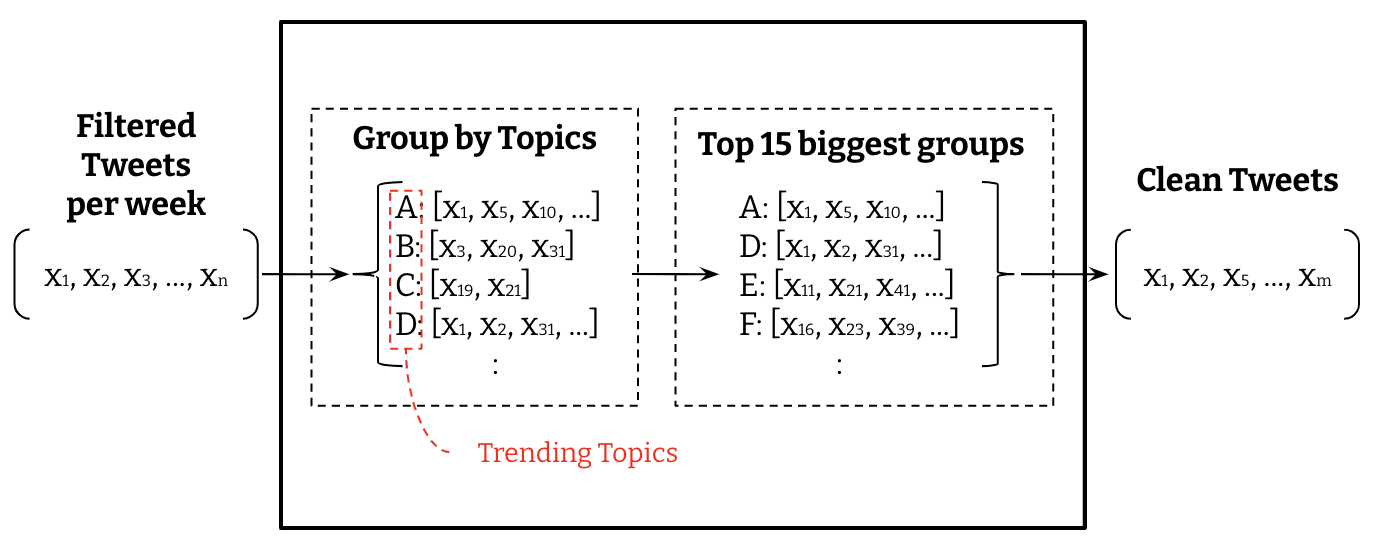
\includegraphics[width=7.5cm]{../figures/tweet-topic/trending_filtering.png}
    \caption{Weekly trend filtering to remove tweets that are irrelevant to the popular topics in each week.}
    \label{fig:trending}
\end{figure}

\begin{figure}[hbt]
    \centering
    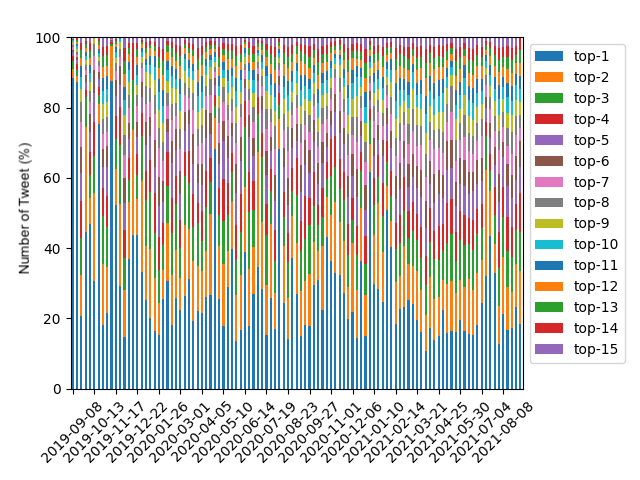
\includegraphics[width=7.5cm]{../figures/tweet-topic/trend.png}
    \caption{Ratio (\%) of tweets in each of top 15 trending keywords for every week.}
    \label{fig:trend_distribution}
\end{figure}

\begin{figure*}[t]
    \centering
    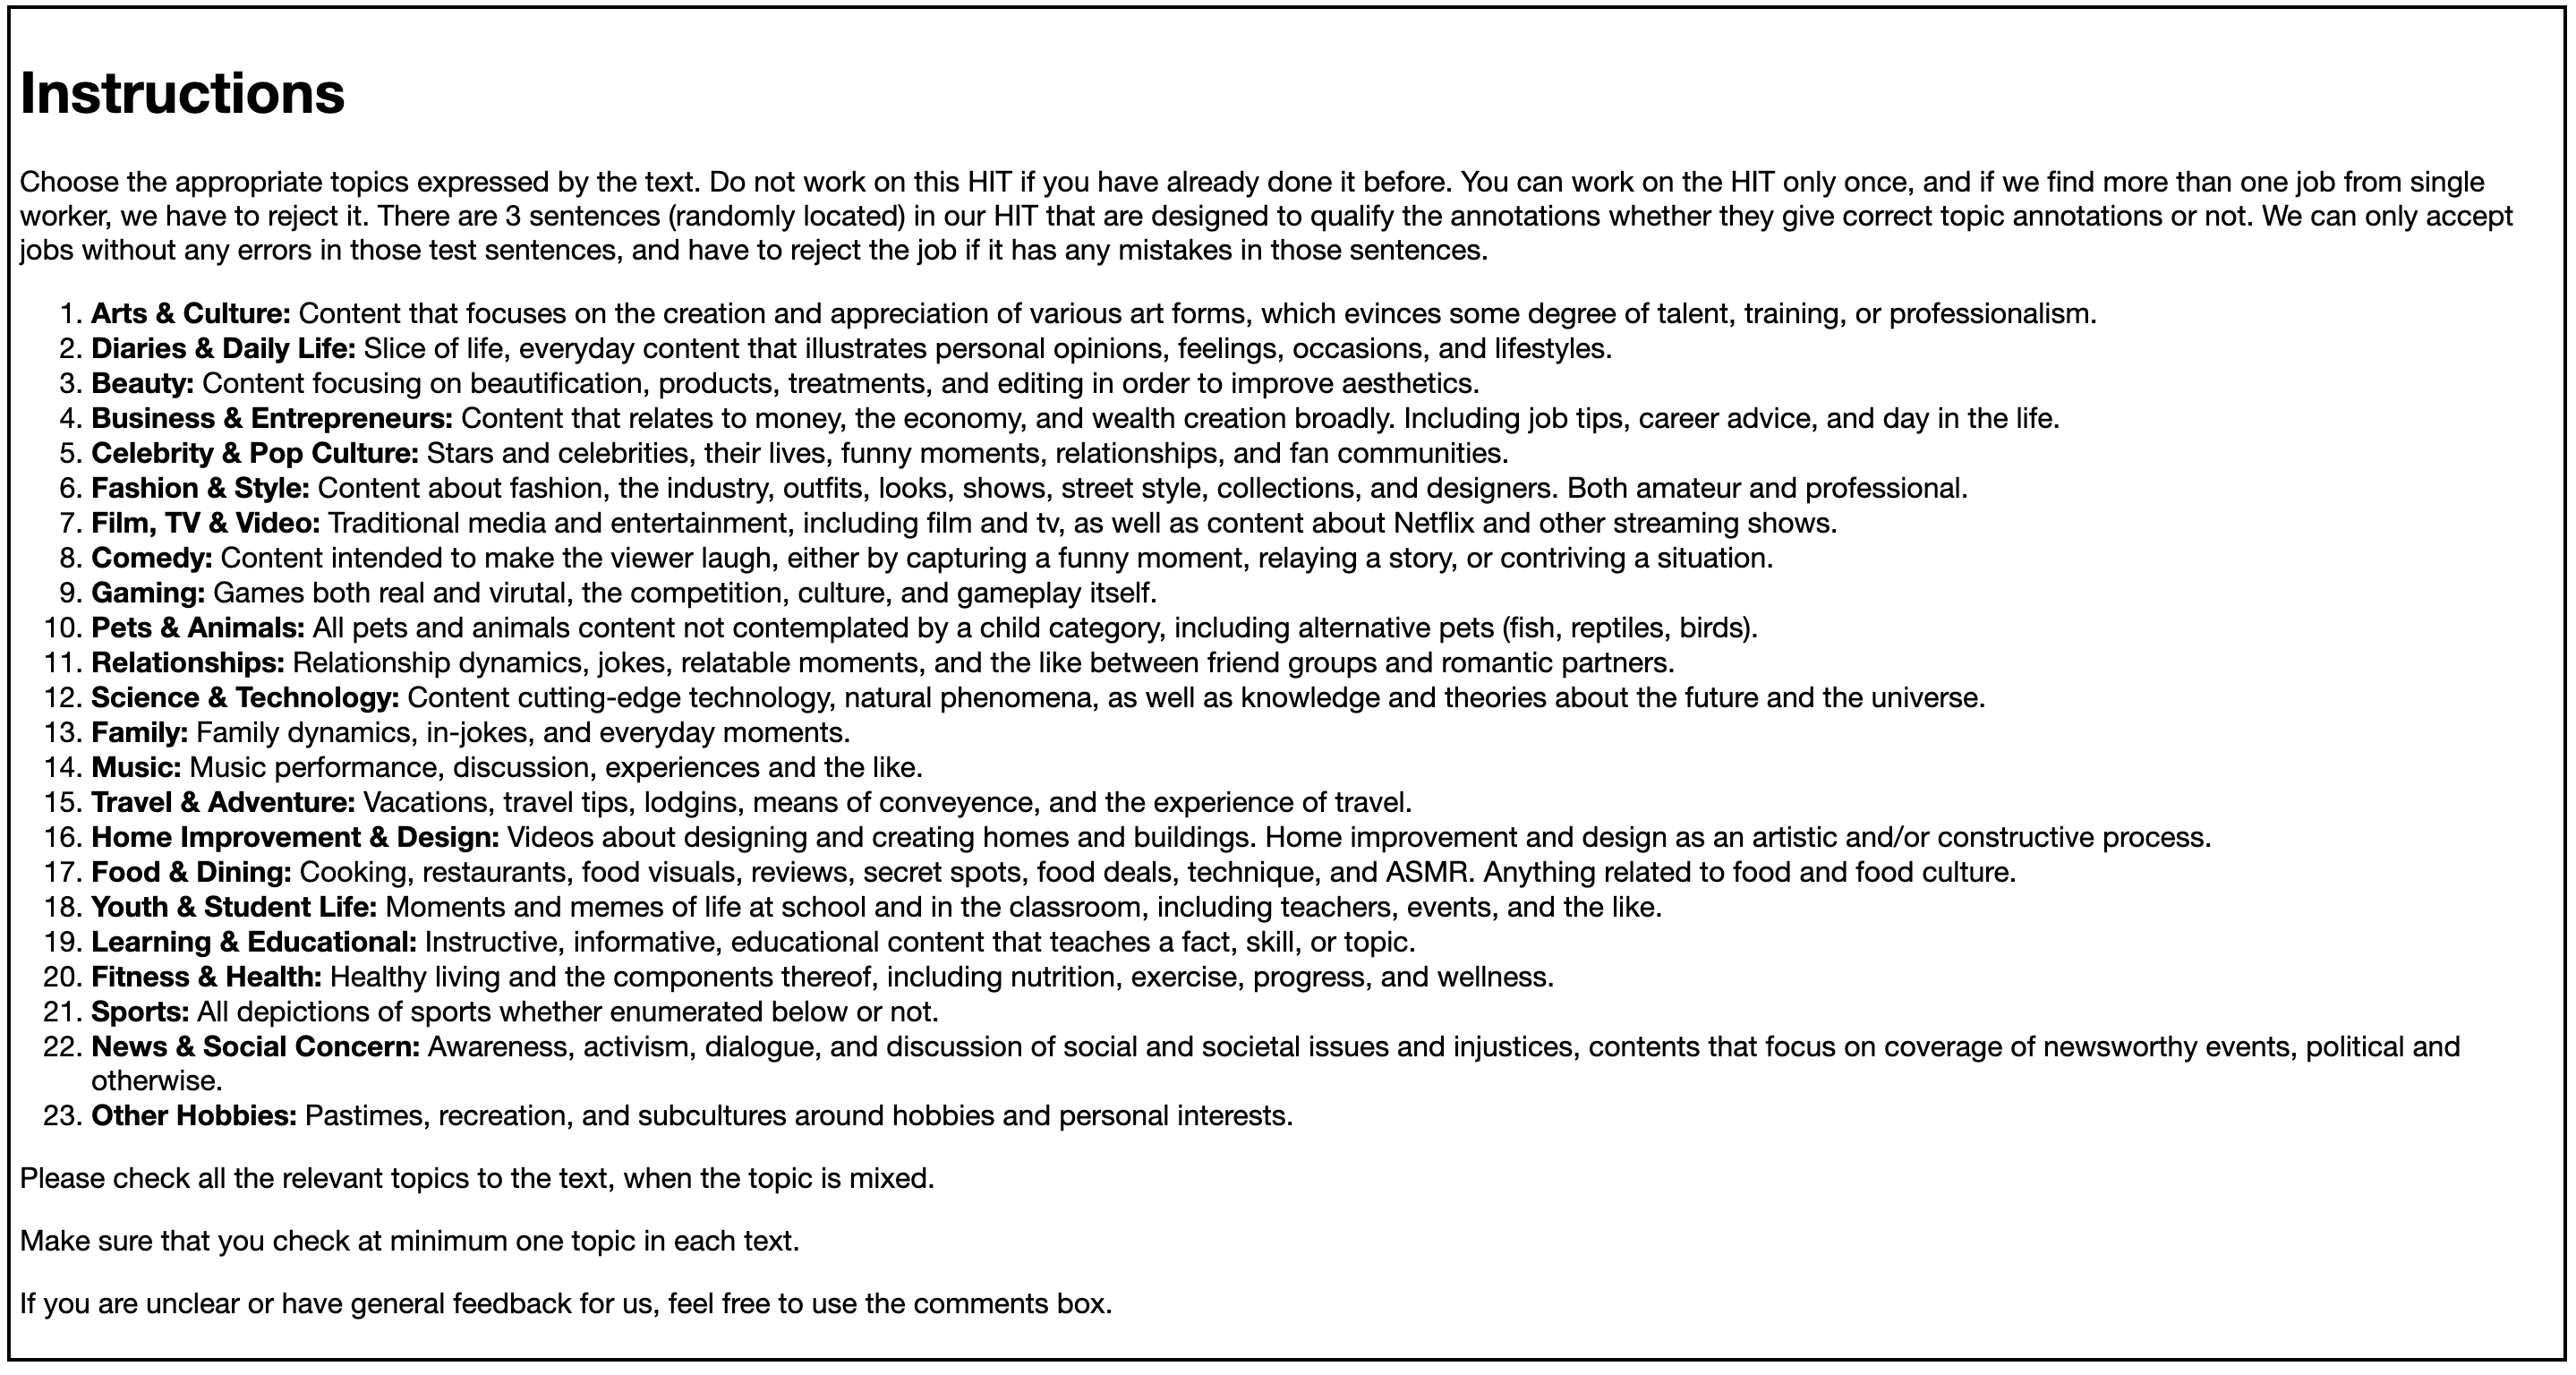
\includegraphics[width=15cm]{../figures/tweet-topic/instruction.png}
    \caption{The instructions shown to the annotators during the annotation phase.}
    \label{fig:instruction}
\end{figure*}

\begin{figure}[t]
    \centering
    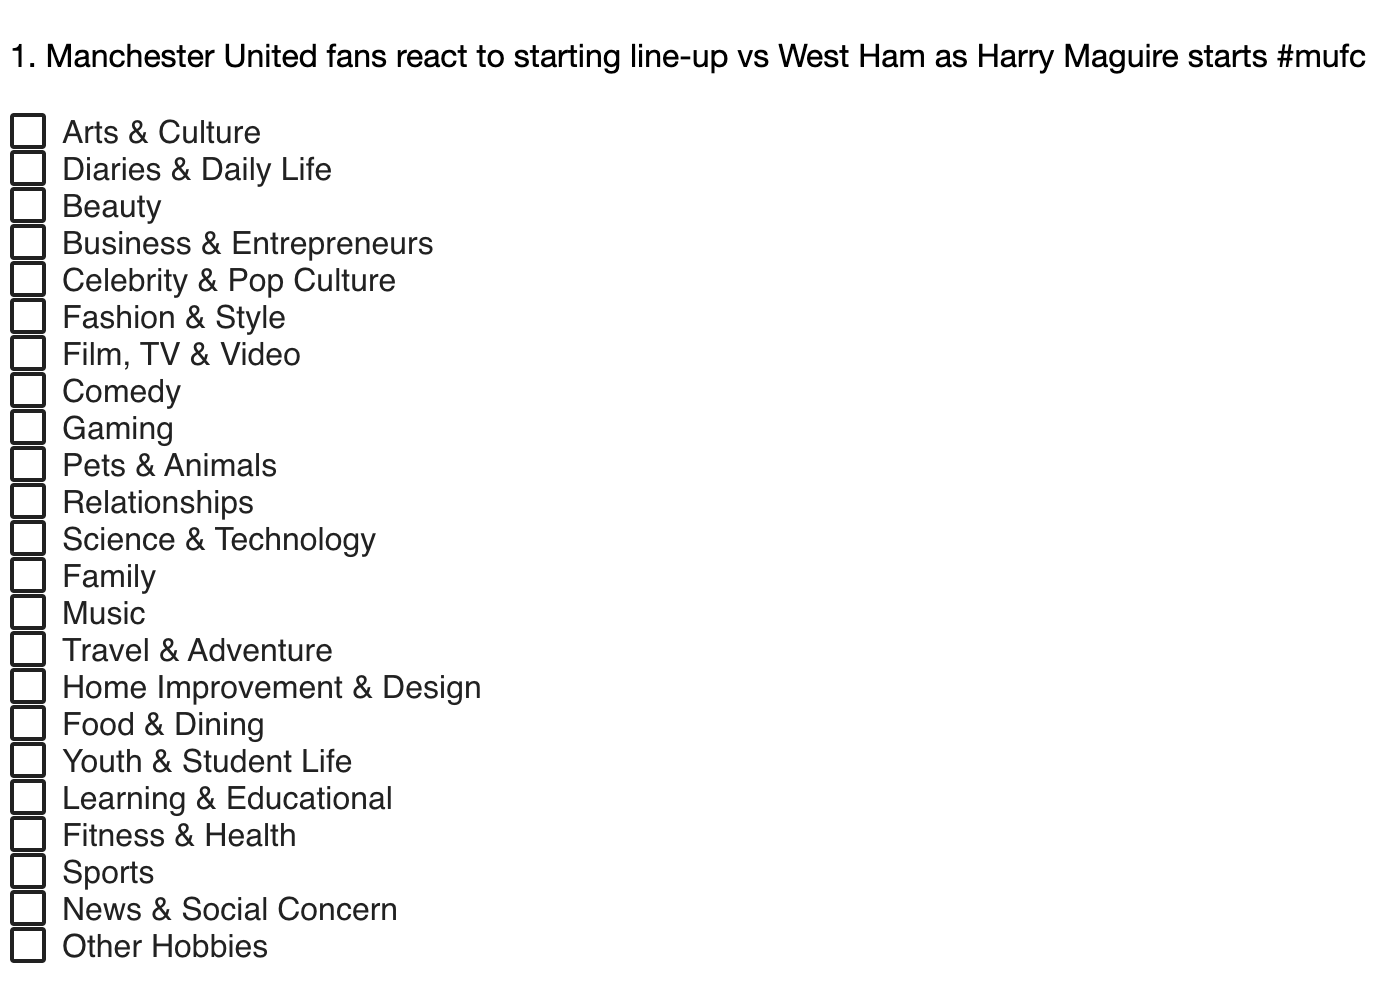
\includegraphics[width=7.5cm]{../figures/tweet-topic/interface.png}
    \caption{Tweet classification annotation interface. Annotators are allowed to select multiple topics.}
    \label{fig:interface}
\end{figure}



\subsection{Evaluation Results}\label{appendix:TweetTopic-evaluation}

\paragraph{Supplementary results.} Table \ref{tab:f1_temporal-random_appendix} displays the F1 scores for each class in the multi-label setting when using the temporal and random split. The best score for each model is highlighted in bold.

\paragraph{Hyperparameters.} Language models are trained using a batch size of 8 for 20 epochs, while utilizing an Adam optimizer \cite{loshchilov2017decoupled} with learning rate $2e^-5$ and a weight decay of $0.01$. Furthermore, an early stop callback  terminates the training process after 3 epochs without performance improvement. Finally, for the single-label experiments cross entropy loss along with a softmax activation function were used, while for the multi-label setting binary cross entropy loss and a sigmoid activation for each of the 19 topics are used.


\paragraph{Analysis by quarter.} In order to get a better understanding of the evolution of the corpus and identify potential performance decays due to temporal differences we inspect the performance of TimeLM-19 in each quarter (i.e., three months) of the temporal's split test-set. Figure \ref{fig:f1_over_time_single} displays the F1 scores of each class (single-label setting) for each quarter of the time period tested. While most topics do not seem to be greatly affected by time, we can indeed observe a performance drop in \textit{arts \& culture}, which is the topic more affected by the temporal variable. Figure \ref{fig:performance_diff_multi} illustrates the relative differences in F1 scores for each class in the multi-label setting, when TimeLM-19 is trained using the temporal split and when trained on the random split.

\paragraph{Confusion matrices.} Figure \ref{fig:confusion_matrix_multi} displays the confusion matrices for TimeLM-19 when trained in the multi-label setting using the temporal split.
 %Figure \ref{fig:f1_over_time_single} illustrates the fluctuation of F1 score for each class through time, when using TimeLM-19 in a single-label setting. Figure \ref{fig:performance_diff_multi} illustrates the relative differences in F1 scores for each class in the multi-label setting, when TimeLM-19 is trained using the temporal split and when trained on the random split. a


 
\begin{table}[t]
\centering
\adjustbox{max width=\textwidth}{%
\begin{tabular}{|l|cc|cc|cc|}
\hline
\multicolumn{1}{|c|}{\multirow{2}{*}{\textbf{Class}}} & \multicolumn{2}{c|}{\textbf{Random}} & \multicolumn{2}{c|}{\textbf{SVM}} & \multicolumn{2}{c|}{\textbf{BERT}} \\ \cline{2-7} 
\multicolumn{1}{|c|}{} & \multicolumn{1}{c|}{\textbf{temp}} & \textbf{rand} & \multicolumn{1}{c|}{\textbf{temp}} & \textbf{rand} & \multicolumn{1}{c|}{\textbf{temp}} & \textbf{rand} \\ \hline
\begin{tabular}[c]{@{}l@{}}arts \& \\ culture\end{tabular} & \multicolumn{1}{c|}{\textbf{8.6}} & 8.3 & \multicolumn{1}{c|}{3.6} & \textbf{27.7} & \multicolumn{1}{c|}{17.8} & \textbf{35.9} \\ \hline
\begin{tabular}[c]{@{}l@{}}business \& \\ entrepreneurs\end{tabular} & \multicolumn{1}{c|}{\textbf{8.7}} & 7.4 & \multicolumn{1}{c|}{18.0} & \textbf{28.7} & \multicolumn{1}{c|}{\textbf{53.3}} & 49.2 \\ \hline
\begin{tabular}[c]{@{}l@{}}celebrity \& \\ pop culture\end{tabular} & \multicolumn{1}{c|}{22.8} & 22.9 & \multicolumn{1}{c|}{22.3} & \textbf{41.7} & \multicolumn{1}{c|}{34.4} & \textbf{54.3} \\ \hline
\begin{tabular}[c]{@{}l@{}}diaries \& \\ daily life\end{tabular} & \multicolumn{1}{c|}{18.2} & \textbf{21.2} & \multicolumn{1}{c|}{25.8} & \textbf{34.4} & \multicolumn{1}{c|}{\textbf{45.2}} & 44.0 \\ \hline
family & \multicolumn{1}{c|}{3.5} & \textbf{6.3} & \multicolumn{1}{c|}{33.9} & \textbf{46.4} & \multicolumn{1}{c|}{47.2} & \textbf{48.3} \\ \hline
\begin{tabular}[c]{@{}l@{}}fashion \& \\ style\end{tabular} & \multicolumn{1}{c|}{\textbf{4.8}} & 4.1 & \multicolumn{1}{c|}{38.4} & \textbf{57.6} & \multicolumn{1}{c|}{52.8} & \textbf{74.8} \\ \hline
\begin{tabular}[c]{@{}l@{}}film tv \& \\ video\end{tabular} & \multicolumn{1}{c|}{\textbf{22.8}} & 22.0 & \multicolumn{1}{c|}{47.3} & \textbf{58.6} & \multicolumn{1}{c|}{62.8} & \textbf{68.2} \\ \hline
\begin{tabular}[c]{@{}l@{}}fitness \& \\ health\end{tabular} & \multicolumn{1}{c|}{6.6} & \textbf{9.3} & \multicolumn{1}{c|}{35.7} & \textbf{36.0} & \multicolumn{1}{c|}{\textbf{53.6}} & 52.2 \\ \hline
\begin{tabular}[c]{@{}l@{}}food \& \\ dining\end{tabular} & \multicolumn{1}{c|}{3.5} & \textbf{4.6} & \multicolumn{1}{c|}{25.0} & \textbf{41.7} & \multicolumn{1}{c|}{\textbf{70.1}} & 68.2 \\ \hline
gaming & \multicolumn{1}{c|}{6.9} & \textbf{7.5} & \multicolumn{1}{c|}{31.8} & \textbf{45.0} & \multicolumn{1}{c|}{57.4} & \textbf{61.2} \\ \hline
\begin{tabular}[c]{@{}l@{}}learning \& \\ educational\end{tabular} & \multicolumn{1}{c|}{4.2} & \textbf{4.5} & \multicolumn{1}{c|}{13.0} & \textbf{13.9} & \multicolumn{1}{c|}{38.2} & \textbf{43.2} \\ \hline
music & \multicolumn{1}{c|}{24.7} & \textbf{25.5} & \multicolumn{1}{c|}{76.1} & \textbf{81.8} & \multicolumn{1}{c|}{83.6} & \textbf{86.0} \\ \hline
\begin{tabular}[c]{@{}l@{}}news \& \\ social concern\end{tabular} & \multicolumn{1}{c|}{39.3} & \textbf{39.9} & \multicolumn{1}{c|}{69.8} & \textbf{76.9} & \multicolumn{1}{c|}{\textbf{83.8}} & \textbf{83.8} \\ \hline
other hobbies & \multicolumn{1}{c|}{\textbf{10.5}} & 9.6 & \multicolumn{1}{c|}{4.2} & \textbf{15.0} & \multicolumn{1}{c|}{\textbf{27.0}} & 23.6 \\ \hline
relationships & \multicolumn{1}{c|}{6.4} & \textbf{7.3} & \multicolumn{1}{c|}{13.7} & \textbf{36.3} & \multicolumn{1}{c|}{30.8} & \textbf{35.2} \\ \hline
\begin{tabular}[c]{@{}l@{}}science \& \\ technology\end{tabular} & \multicolumn{1}{c|}{8.3} & \textbf{9.3} & \multicolumn{1}{c|}{17.4} & \textbf{35.8} & \multicolumn{1}{c|}{45.9} & \textbf{50.3} \\ \hline
sports & \multicolumn{1}{c|}{\textbf{36.6}} & 34.8 & \multicolumn{1}{c|}{82.2} & \textbf{89.1} & \multicolumn{1}{c|}{93.1} & \textbf{93.2} \\ \hline
\begin{tabular}[c]{@{}l@{}}travel \& \\ adventure\end{tabular} & \multicolumn{1}{c|}{2.2} & \textbf{3.5} & \multicolumn{1}{c|}{\textbf{17.7}} & 9.8 & \multicolumn{1}{c|}{\textbf{21.7}} & 20.6 \\ \hline
\begin{tabular}[c]{@{}l@{}}youth \& \\ student life\end{tabular} & \multicolumn{1}{c|}{1.7} & \textbf{2.9} & \multicolumn{1}{c|}{2.9} & \textbf{12.4} & \multicolumn{1}{c|}{33.3} & \textbf{44.6} \\ \hline
\textbf{samples avg} & \multicolumn{1}{c|}{13.8} & \textbf{14.3} & \multicolumn{1}{c|}{57.0} & \textbf{63.7} & \multicolumn{1}{c|}{\textbf{70.3}} & 72.0 \\ \hline
\textbf{macro avg} & \multicolumn{1}{c|}{12.6} & \textbf{13.2} & \multicolumn{1}{c|}{30.5} & \textbf{41.5} & \multicolumn{1}{c|}{50.1} & \textbf{54.6} \\ \hline
\end{tabular}
}
\caption{  Average F1 scores for the multi-label setting when using temporal (temp) and random (rand) split. Highlighted with bold is the best score for each model}
\label{tab:f1_temporal-random_appendix}
\end{table}

\begin{figure}[hbt!]
    \centering
    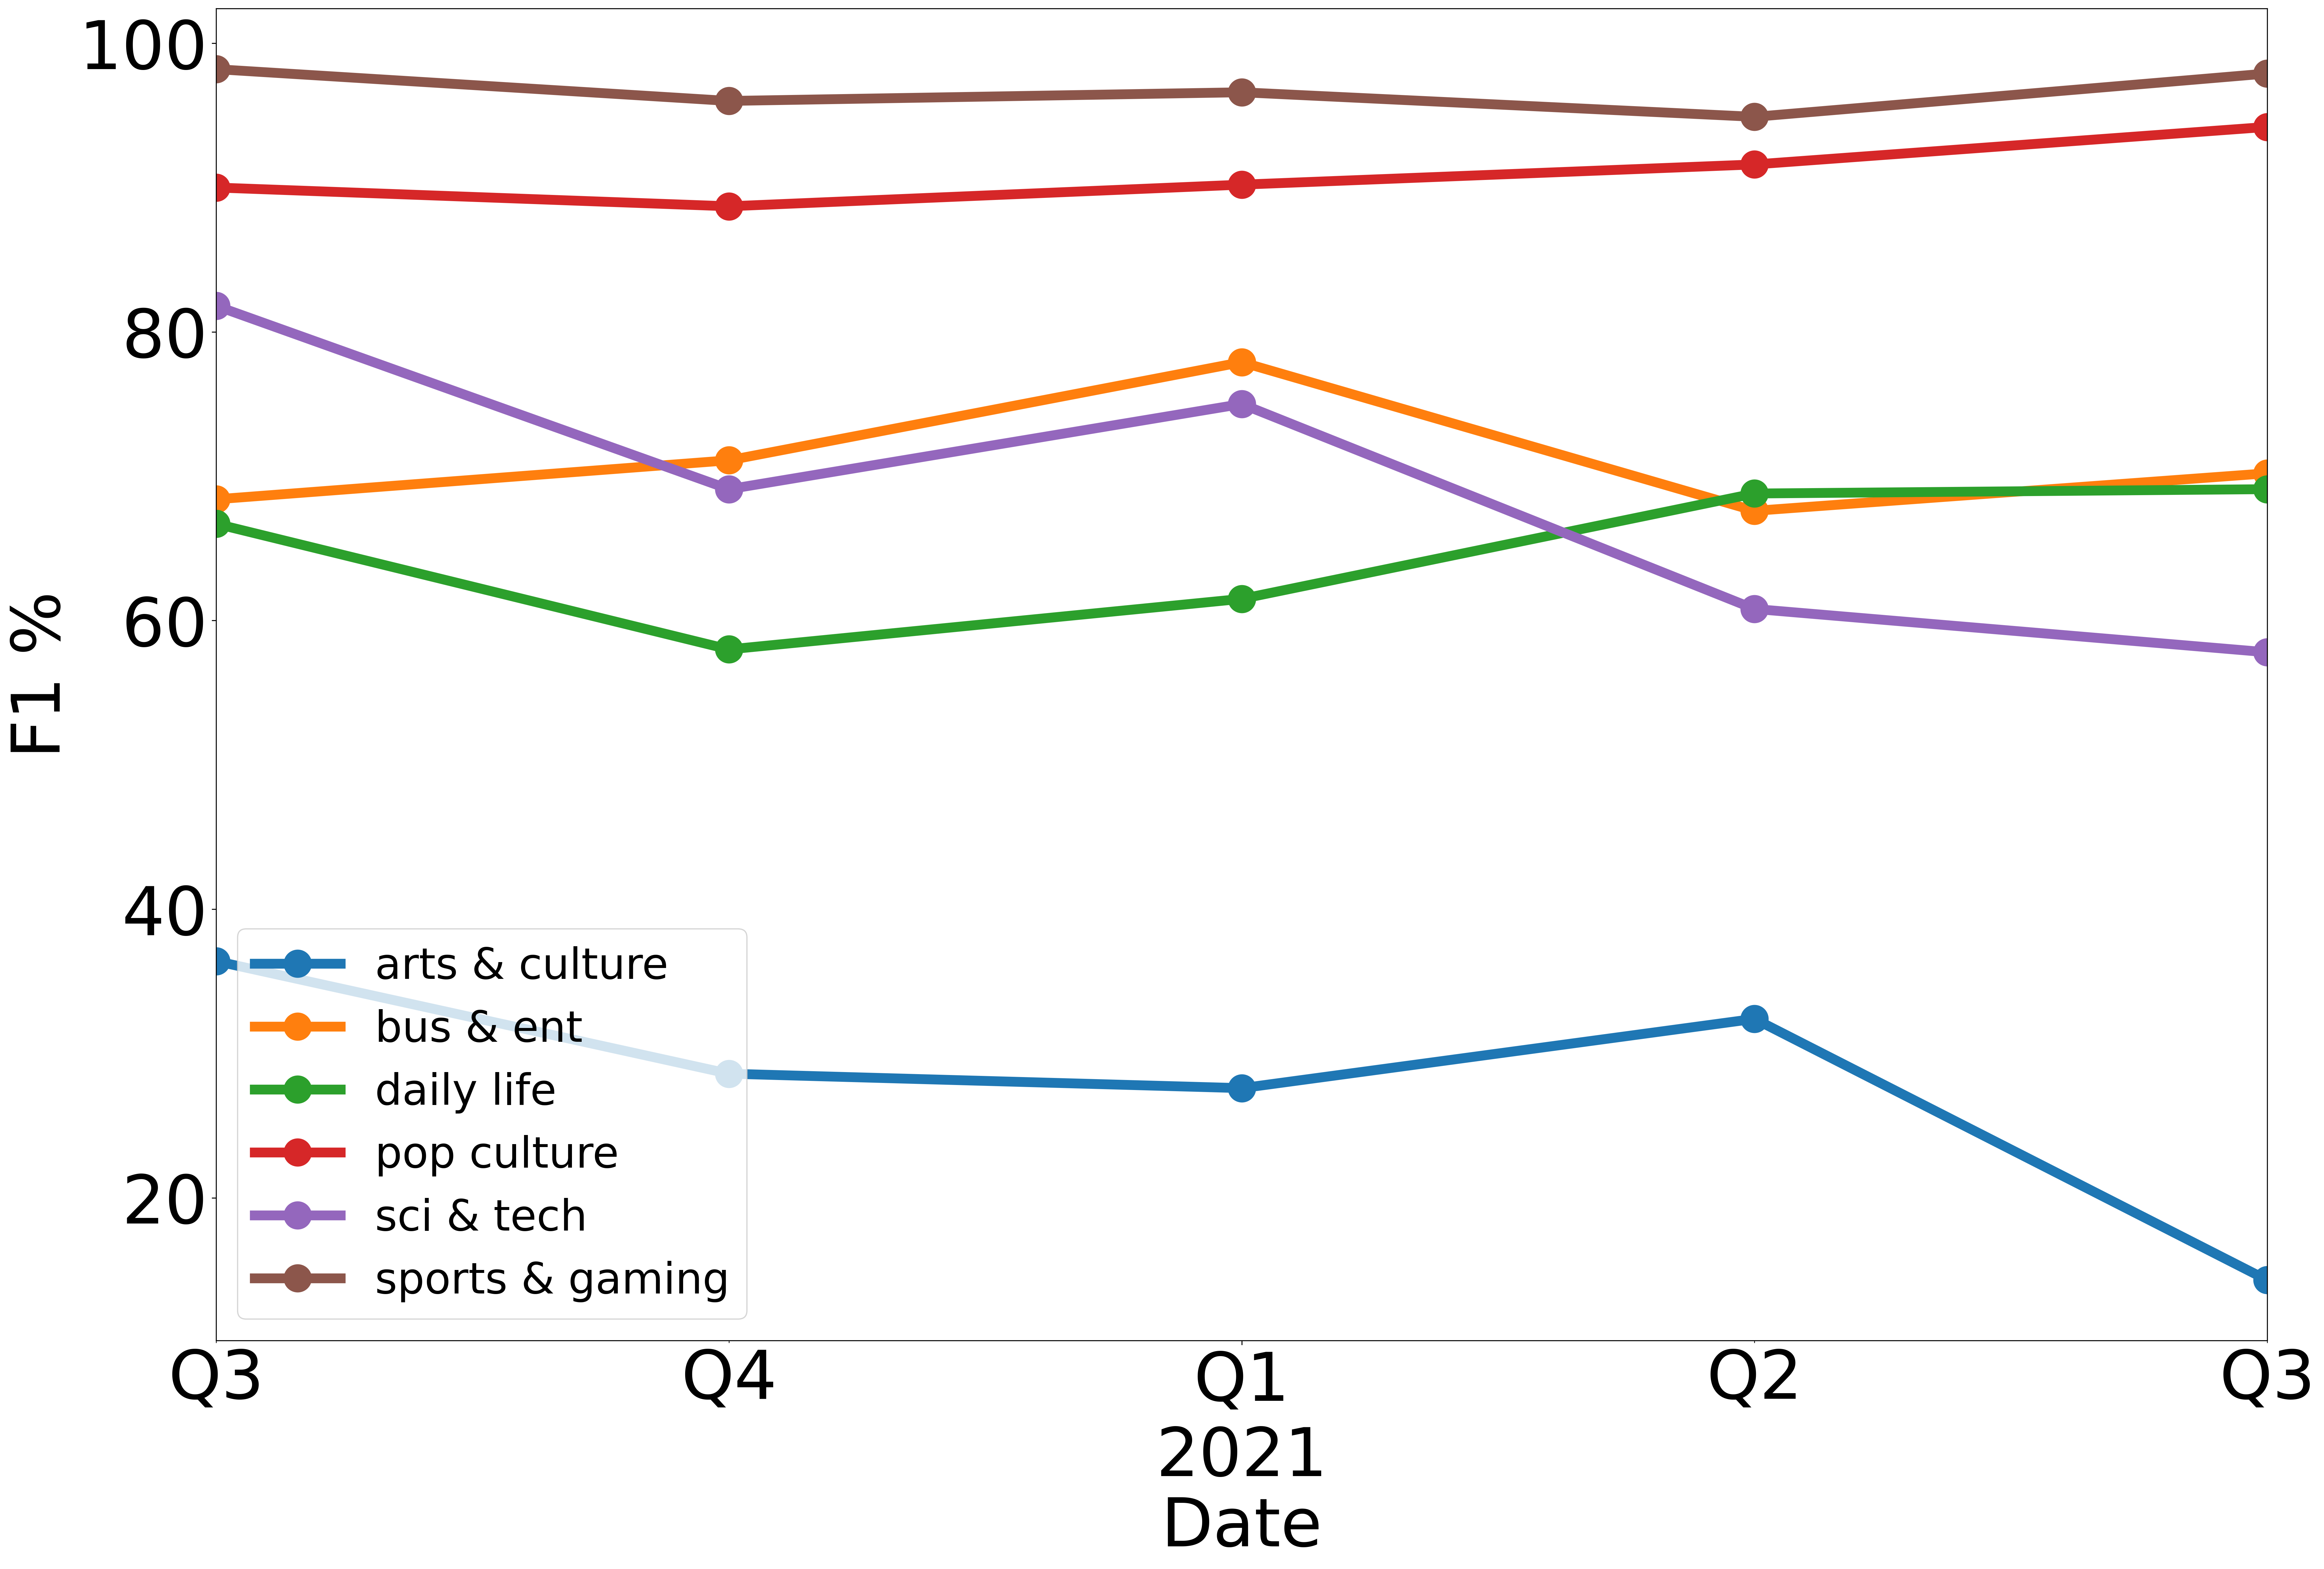
\includegraphics[width=7.5cm]{../figures/tweet-topic/troberta2019_temp_decay.png}
    \caption{F1 performance of TimeLM-19 through time (single-label setting).}
    \label{fig:f1_over_time_single}
\end{figure}


\begin{figure}[t]
    \centering
    \includegraphics[width=7.5cm]{../figures/tweet-topic/performance_diff.png}
    \caption{Relative (\%) differences in F1 scores when \textit{TimeLM-19} is trained in a temporal and in a random setting for the multi-label setting. Negative values indicate that when using the temporal split the model's performance decreases. }
    \label{fig:performance_diff_multi}
\end{figure}



\begin{figure*}[t]
    \centering
    \includegraphics[width=.9\textwidth]{../figures/tweet-topic/troberta2019_cm_multi.png}
    \caption{Confusion-matrix of TimeLM-19 (multi-label setting).}
    \label{fig:confusion_matrix_multi}
\end{figure*}


\clearpage



\section{XTopic}\label{appendix:Xtopic}


\subsection{Annotation Guidelines}
\label{appendix:XTopic-guidelines}
Below we provide the guidelines provided to the coders of each language.
\subsubsection{English}
Choose the appropriate topics expressed by the text. 
You can work on this task only once,  multiple tasks from the same annotators will be rejected. 
Some simple sentences are designed to verify the quality of  the annotations.. We will reject tasks where these simple test questions are not correct. 

For privacy reasons and to make the annotation easier, all non-verified user mentions are represented as \{\{USER\}\} and all URL entries as \{\{URL\}\}.

1. Arts \& Culture: Content about art forms, which evinces some degree of talent, training, or professionalism.

2. Business \& Entrepreneurs: Content that relates to money, the economy, and wealth creation broadly. Including job tips, career advice, and day in the life.

3. Celebrity \& Pop Culture: Stars and celebrities, their lives, funny moments, relationships, and fan communities.

4. Diaries \& Daily Life: Slice of life, everyday content that illustrates personal opinions, feelings, occasions, and lifestyles.

5. Family: Family dynamics, in-jokes, and everyday moments.

6. Fashion \& Style: Content about fashion, outfits, looks, shows, street style, collections, and designers. Both amateur and professional.

7. Film, TV \& Video: Traditional media and entertainment, including film, and tv, as well as content about Netflix and other streaming shows.

8. Fitness \& Health: Healthy living and the components thereof, including nutrition, exercise, progress, and wellness.

9. Food \& Dining: Anything related to food and food culture. Cooking, restaurants, food, reviews, technique, and ASMR. 

10. Learning \& Educational: Instructive, informative, educational content that teaches a fact, skill or topic.

11. News \& Social Concern: Awareness, activism, and discussion of societal issues and injustices contents that focus on coverage of newsworthy events, political and otherwise.

12. Relationships: Relationship dynamics, jokes, relatable moments, and the like between friend groups and romantic partners.

13. Science \& Technology: Content related to technology, natural phenomena, as well as knowledge and theories about the future and the universe.

14. Youth \& Student Life: Moments and memes of life at school and in the classroom, including teachers, events, and the like.

15. Music: Music performance, discussion, experiences and the like.

16. Gaming: Video games related content, gameplay, competition, culture and other games (e.g. board games). 

17. Sports: All depictions of sports (e.g. football, baseball, cricket, tennis, etc.). 

18. Travel \& Adventure: Vacations, travel tips, lodgings, means of conveyance, and the experience of travel.

19. Other Hobbies: Hobbies and personal interests not included in the topics above.

Multiple topics are allowed, please check ALL the relevant topics to the text, when the topic is mixed.
Make sure that you check at least one topic in each text.
 
Do you understand the instructions?

\subsubsection{Spanish}
Elija los temas apropiados expresados por el texto.
Sólo puede trabajar en esta tarea una vez, se rechazarán varias tareas de los mismos anotadores.
Algunas oraciones simples están diseñadas para verificar la calidad de las anotaciones. Rechazaremos las tareas en las que estas preguntas de prueba simples no sean correctas.

Por motivos de privacidad y para facilitar la anotación, todas las menciones de usuarios no verificados se representan como \{\{USUARIO\}\} y todas las entradas de URL como \{\{URL\}\}.

1. Arte y cultura: Contenido sobre formas de arte que demuestre algún grado de talento, capacitación o profesionalismo.

2. Negocios y emprendedores: Contenido relacionado con el dinero, la economía y la creación de riqueza en general. Incluyendo consejos de trabajo, de carrera u otros.

3. Celebridades y cultura pop: Estrellas y celebridades, sus vidas, momentos divertidos, relaciones y comunidades de admiradores.

4. Diarios y vida diaria: Contenido cotidiano y de vida diaria que ilustra opiniones personales, sentimientos, eventos y estilos de vida.

5. Familia: Dinámicas y referencias familiares, momentos cotidianos.

6. Moda y estilo: Contenido sobre moda, atuendos, looks, desfiles, estilo callejero, colecciones y diseñadores. Tanto amateur como profesional.

7. Cine, televisión y video: Medios tradicionales y de entretenimiento, incluidos cine y televisión, así como contenido sobre programas de streaming.

8. Estado físico y salud: Estilos de vida saludable y similar, incluida la nutrición, el ejercicio, el progreso y el bienestar.

9. Food \& Dining: Todo lo relacionado con la comida y la cultura gastronómica. Cocina, restaurantes, comida, reseñas, recetas y otros.

10. Aprendizaje y educación: Contenido instructivo, informativo y educativo para enseñar hechos, habilidades o temáticas.

11. Noticias e interés social: Conciencia, activismo y debate sobre problemas sociales y contenidos de injusticias que se centran en la cobertura de eventos de interés periodístico, políticos y de otro tipo.

12. Relaciones: Dinámicas de relación, bromas, momentos identificables y similares entre grupos de amigos y parejas románticas.

13. Ciencia y Tecnología: Contenido de tecnología, fenómenos naturales, así como conocimientos y teorías sobre el futuro y el universo.

14. Juventud y Vida Estudiantil: Momentos y memes de la vida en la escuela y en clase, incluidos maestros, eventos y similares.

15. Música: Interpretación musical, discusión, experiencias y similares.

16. Juegos: Contenido relacionado con videojuegos, juegos de rol, competición y otros juegos (por ejemplo, juegos de mesa).

17. Deportes: Todo lo relacionado con el deporte (por ejemplo, fútbol, béisbol, atletismo, tenis, etc.).

18. Viajes y aventuras: Vacaciones, consejos de viaje, alojamiento, medios de transporte y experiencias de viaje.

19. Otros pasatiempos: Pasatiempos, hobbies e intereses personales no incluidos en los temas anteriores.

Se permiten múltiples temas, marque TODOS los temas relevantes para el texto (puede ser más de uno cuando la temática es variada).

Asegúrese de marcar al menos un tema en cada texto.
 
¿Entiendes las instrucciones?

\subsubsection{Japanese}
\begin{CJK*}{UTF8}{min}
インストラクション

ツイートの文章に対し、適切なトピックをリストから選んでください。このアノテーションには一度しか参加することはできません。同じアノテーターから複数のアノテーションがあった場合、それは受理されることはありませんので注意してください。アノテーションの品質保持のためアノテーションの中にはいくつか簡単な例題があり、それらを間違えた場合もアノテーションは受理されません。

ツイートのプライバシー保護のため、non-verified user name 及び web url はマスキングされています。

1. アート\&カルチャー: アートや文化など芸術性や専門性の高い物に関するツイート。

2. ビジネス: 経済やビジネス、金融などに関わるツイート。キャリア形成や転職情報なども含まれます。

3. 芸能: 芸能人やそれらが主催するイベントなどに関するツイート。

4. 日常: 日々の出来事などの日常的な事柄に関するツイート。

5. 家族: 家族に関するツイート

6. ファッション: ストリートスナップやデザイン、ファッションに関するツイート。

7. 映画\&ラジオ: TVやラジオ、映画などのエンタメ等に関するツイート。

8. フィットネス\&健康: 栄養、フィットネスなどに関するツイート。

9. 料理: 料理やレストランなど食に関するツイート

10. 教育関連: 教育に関するツイート。

11. 社会: 社会情勢やそれに通ずるニュース、政治などに関するツイート。

12. 人間関係: パートナーシップや恋人との関係性などに関するツイート。

13. サイエンス: IT含むサイエンスに関するツイート。

14. 学校: 学校での出来事や行事に関するツイート。

15. 音楽: 音楽フェスや音楽そのものに関するツイート。

16. ゲーム: ゲーム（オンラインゲームやビデオゲーム等）に関するツイート。

17. スポーツ: スポーツに関するツイート。

18. 旅行: 旅行に関するツイート。

19. その他: その他、趣味や個人の嗜好に関するツイート。
一つのツイートに対し複数のラベルの付与が可能になってます。

少なくとも一つのトピックを選んでください。
 
インストラクションは理解できましたでしょうか？
\end{CJK*}

\subsubsection{Greek}
\selectlanguage{greek}
Επιλέξτε τα κατάλληλα θέματα που εκφράζει το κείμενο.

Μπορείτε να εργαστείτε σε αυτήν την εργασία μόνο μία φορά, πολλές εργασίες από τους ίδιους σχολιαστές θα απορριφθούν. Ορισμένες απλές προτάσεις έχουν σχεδιαστεί για να επαληθεύουν την ποιότητα των σχολιασμών. Θα απορρίψουμε εργασίες όπου αυτές οι απλές ερωτήσεις δοκιμής δεν είναι σωστές.
Για λόγους απορρήτου και για να γίνει ευκολότερος ο σχολιασμός, όλες οι μη επαληθευμένες αναφορές χρηστών αντιπροσωπεύονται ως \selectlanguage{english} \{\{USER\}\} \selectlanguage{greek} και όλες οι \selectlanguage{english} URL \selectlanguage{greek} ως \selectlanguage{english} \{\{URL\}\}.

\selectlanguage{greek}
1. Τέχνες \& Πολιτισμός: Περιεχόμενο για μορφές τέχνης, το οποίο δείχνει κάποιο βαθμό ταλέντου, κατάρτισης ή επαγγελματισμού.

2. Επιχειρήσεις \& Επιχειρηματίες: Περιεχόμενο που σχετίζεται γενικά με τα χρήματα, την οικονομία και τη δημιουργία πλούτου. Συμπεριλαμβάνονται συμβουλές για δουλειά, συμβουλές σταδιοδρομίας, κτλ.

3. Διασημότητες \& Ποπ κουλτούρα: Αστέρια και διασημότητες, η ζωή τους, αστείες στιγμές, σχέσεις και κοινότητες θαυμαστών.

4. Ημερολόγια \& Καθημερινή ζωή: Στιγμές της ζωής, καθημερινό περιεχόμενο που απεικονίζει προσωπικές απόψεις, συναισθήματα, περιστάσεις και τρόπους ζωής.

5. Οικογένεια: Δυναμική της οικογένειας, αστεία και καθημερινές στιγμές.

6. Μόδα \& Στυλ: Περιεχόμενο σχετικά με τη μόδα, τα ρούχα, τις εμφανίσεις, τις επιδείξεις, το street style, τις συλλογές και τους σχεδιαστές. Ερασιτεχνική και επαγγελματική.

7. Ταινίες, τηλεόραση \& βίντεο: Παραδοσιακά μέσα και ψυχαγωγία, συμπεριλαμβανομένων ταινιών και τηλεόρασης, καθώς και περιεχόμενο για το Netflix και άλλες εκπομπές ροής.

8. Γυμναστική \& Υγεία: Υγιεινή ζωή και τα συστατικά της, συμπεριλαμβανομένης της διατροφής, της άσκησης, της προόδου και της ευεξίας.

9. Φαγητό \& Δείπνο: Οτιδήποτε σχετίζεται με το φαγητό και την κουλτούρα του φαγητού. Μαγειρική, εστιατόρια, φαγητό, κριτικές, τεχνική και \selectlanguage{english}ASMR\selectlanguage{greek}.

10. Μάθηση \& Εκπαίδευση: Εκπαιδευτικό, ενημερωτικό, εκπαιδευτικό περιεχόμενο που διδάσκει ένα γεγονός, μια δεξιότητα ή ένα θέμα.

11. Ειδήσεις \& Κοινωνία: Ευαισθητοποίηση, ακτιβισμός και συζήτηση για κοινωνικά ζητήματα και αδικίες, περιεχόμενα που εστιάζουν στην κάλυψη γεγονότων άξιων ειδήσεων, πολιτικών και άλλων.

12. Σχέσεις: Δυναμική σχέσεων, αστεία, συγγενείς στιγμές και άλλα παρόμοια μεταξύ ομάδων φίλων και ρομαντικών συντρόφων.

13. Επιστήμη \& Τεχνολογία: Περιεχόμενο αιχμής τεχνολογίας, φυσικά φαινόμενα, καθώς και γνώση και θεωρίες για το μέλλον και το σύμπαν.

14. Νεανική \& Φοιτητική ζωή: Στιγμές και memes της ζωής στο σχολείο και στην τάξη, συμπεριλαμβανομένων δασκάλων, εκδηλώσεων και παρόμοια.

15. Μουσική: Μουσική παράσταση, συζήτηση, εμπειρίες και παρόμοια.

16. Παιχνίδια: περιεχόμενο σχετικό με βιντεοπαιχνίδια, παιχνίδι, ανταγωνισμό, πολιτισμό και άλλα παιχνίδια (π.χ. επιτραπέζια παιχνίδια).

17. Αθλητισμός: Όλες οι απεικονίσεις αθλημάτων (π.χ. ποδόσφαιρο, μπέιζμπολ, τένις).

18. Ταξίδια \& Περιπέτεια: Διακοπές, ταξιδιωτικές συμβουλές, καταλύματα, μεταφορικά μέσα και η εμπειρία του ταξιδιού.

19. Άλλα χόμπι: Χόμπι και προσωπικά ενδιαφέροντα που δεν περιλαμβάνονται στα παραπάνω θέματα.

Επιτρέπονται πολλά θέματα, παρακαλούμε ελέγξτε ΟΛΑ τα σχετικά θέματα στο κείμενο, όταν τα θέματα αναμιγνύονται.
Βεβαιωθείτε ότι έχετε επιλέξει τουλάχιστον ένα θέμα σε κάθε κείμενο.

Καταλαβαίνετε τις οδηγίες;

\selectlanguage{english}

\subsection{Models \& Dataset}
\label{appendix:XTopic-models}

\subsubsection{Dataset}\label{appendix:Xtopic-dataset}
Table \ref{tab:preprocessing_steps} displays the number of remaining tweets in each preprocessing step for each language. The steps are: 1) language detection (ftext), 2) removal of incomplete/abusing tweets, 3) deduplication, 4) removal of tweets with high ammount of mentions and emojis, and 5) removal of tweets containing URLs.

\begin{table*}[]
\resizebox{\textwidth}{!}{
\begin{tabular}{c|cccccc}
   & Total   & ftext   & incomplete/abusing & deduplication & mentions/emojis & URLS    \\ \hline
en & 225,400 & 217,491 & 208,442            & 193,560       & 178,841         & 81,929  \\ \hline
es & 225,350 & 218,163 & 197,617            & 186,266       & 178,060         & 110,669 \\ \hline
ja & 455,846 & 455,846 & 438,080            & 407,589       & 383,669         & 207,472 \\ \hline
gr & 225,300 & 218,461 & 214,031            & 206,147       & 203,947         & 30,858 
\end{tabular}}
\caption{Number of remaining tweets for each preprocessing step for every language.}
\label{tab:preprocessing_steps}
\end{table*}

Figure \ref{fig:overlap} displays the overlap between topics across all languages.

\begin{figure}
    \centering
    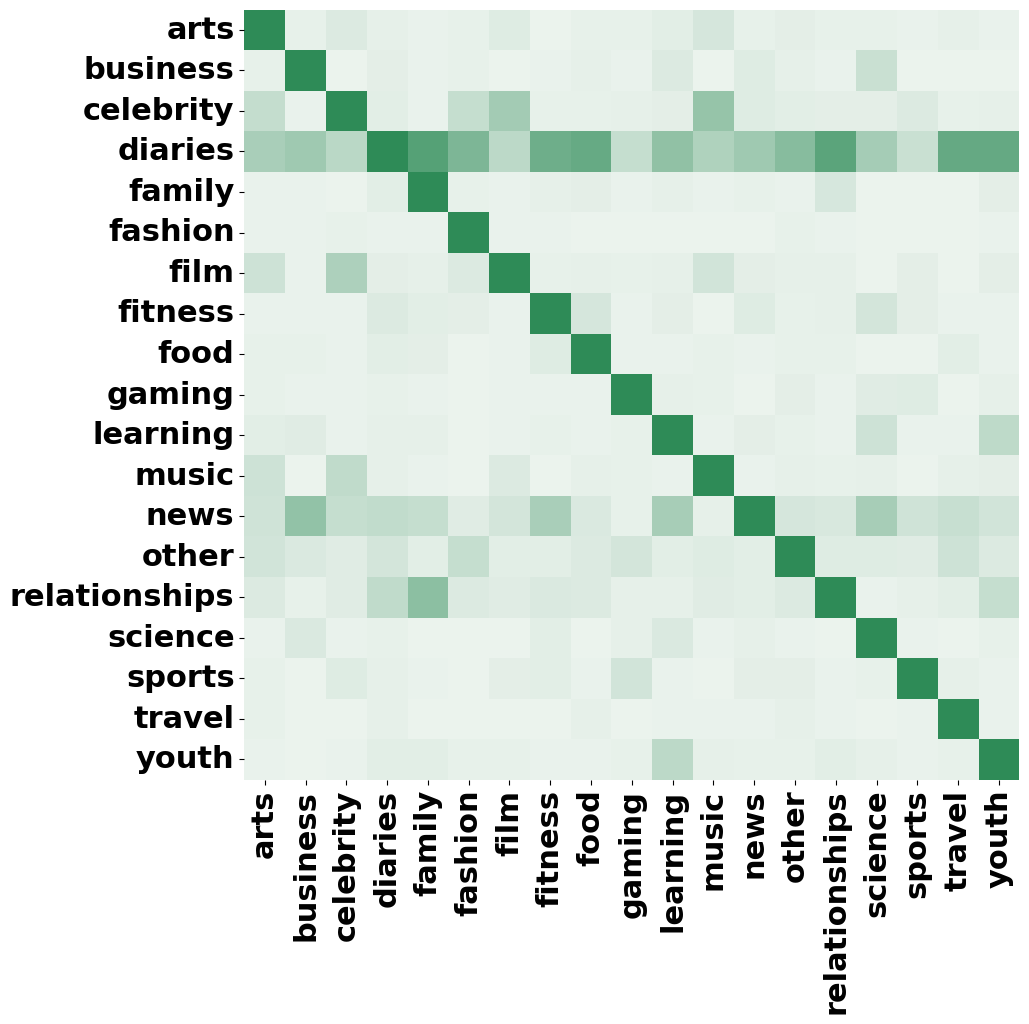
\includegraphics[width=1\linewidth]{../figures/x-topic/overlap.png}
    \caption{Overlap between topics across all languages. Darker colour indicates higher overlap}
    \label{fig:overlap}
\end{figure}

\subsubsection{Models}
In total we estimate 168 hours used for the training of  \textit{bernice, xlm\_r}, and \textit{xlm\_t} models using a NVIDIA GeForce RTX 4090  GPU and 20 hours for \textit{bloomz} and \textit{mt0} models using an  NVIDIA Quadro RTX 8000 GPU.
Table \ref{tab:parameters} provides details for the models used in our experiments.

\begin{table}[ht]
\centering
\begin{tabular}{|l|l|}
\hline
\textbf{Model}         & \textbf{Parameters} \\ \hline
Bernice                              & 125M                  \\ \hline
XLM-R(T) base                           & 270M                  \\ \hline
XLM-R(T) large                           & 550M  \\ \hline
bloomz & 7B \\ \hline
mt0                           & 13B  \\ \hline
chat-gpt                      &  175B (approximate)     \\ \hline
\end{tabular}
\caption{Number of Parameters in different language models used.}
\label{tab:parameters}
\end{table}

\subsubsection{Prompts}
\label{appendix:XTopic-prompts}
Below we present the prompt used in the zero and few-shot settings of our experiments. The prompt used were similar to the ones used in \citet{muennighoff2022crosslingual}.



\noindent Classify the text "\{\{ tweet \}\}" into the following topics:
- \{\{ answer\_choices | join('\textbackslash n- ') \}\}

\noindent Topics:

\subsection{Topics Abbreviation}
\label{appendix:XTopic-topic_abbreviations}
Below we provide the abbreviations of topics used in the paper:

Arts \& Culture: arts

Business \& Entrepreneurs: business

Celebrity \& Pop Culture: celebrity

Diaries \& Daily Life: diaries

Family: family

Fashion \& Style: fashion

Film, TV \& Video: film

Fitness \& Health: fitness

Food \& Dining: food

Learning \& Educational: learning

News \& Social Concern: news

Relationships: relationships

Science \& Technology: science

Youth \& Student Life: youth

Music: music

Gaming: gaming

Sports: sports

Travel \& Adventure: travel

Other Hobbies: other


\subsection{}{Extended Results}
\label{appendix:XTopic-results}

Figure \ref{fig:best_f1}, displays the scores achieved by the overall best-performing model, \textit{xlm\_t-large}, in each language and setting.

Tables \ref{tab:xlmt-details} and \ref{tab:gpt-4o-details} display detail results for the two best performing models, \textit{xlmt\_large} , trained on \textit{TweetTopic} and \textit{All languages}, and  \textit{gpt-4o}, in the \textit{few-shot} setting, respectively. The precision, recall, and f1 scores for each topic in every language are displayed. 


\begin{table}[h!]
    \centering
    \begin{tabular}{lcccc}
        \hline
        \textbf{Metric} & \textbf{en} & \textbf{es} & \textbf{ja} & \textbf{gr} \\
        \hline
        macro & 6.4 & 6.5 & 1.5 & 5.0 \\
        micro & 30.4 & 44.0 & 8.3 & 7.4 \\
        \hline
    \end{tabular}
    \caption{Macro and F1 scores for each language for the SuperCTM model.}
    \label{tab:ctopic}
\end{table}

\begin{figure*}
    \centering
    \scalebox{0.9}{
    \centering
    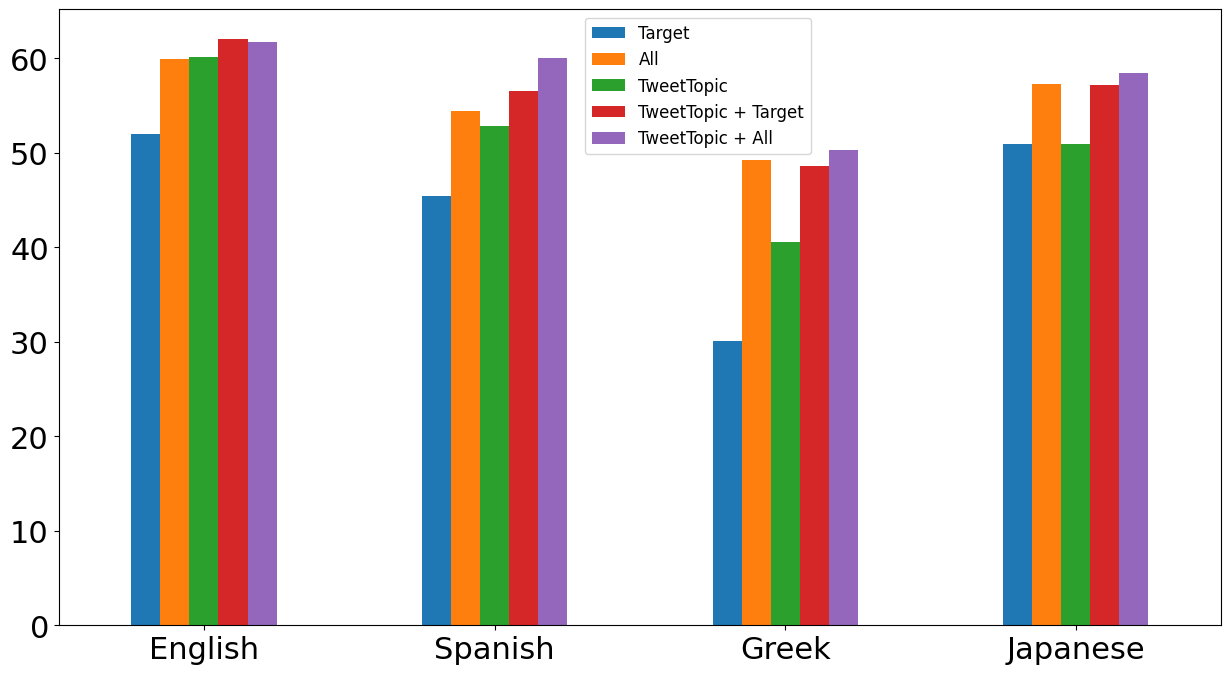
\includegraphics[width=\linewidth]{../figures/x-topic/best_models.png}}
    \caption{F1 scores (macro average) of the best overall performing model (\textit{xlmt\_large}) in each setting and language.}
    \label{fig:best_f1}
\end{figure*}

\begin{table*}[]
\resizebox{\textwidth}{!}{
\begin{tabular}{l|ccc|ccc|ccc|ccc}
\textbf{} &
  \multicolumn{3}{c|}{\textbf{en}} &
  \multicolumn{3}{c|}{\textbf{es}} &
  \multicolumn{3}{c|}{\textbf{gr}} &
  \multicolumn{3}{c}{\textbf{ja}} \\ \hline
\textit{topic} &
  \textbf{Pr} &
  \textbf{Rec} &
  \textbf{F1} &
  \textbf{Pr} &
  \textbf{Rec} &
  \textbf{F1} &
  \textbf{Pr} &
  \textbf{Rec} &
  \textbf{F1} &
  \textbf{Pr} &
  \textbf{Rec} &
  \textbf{F1} \\ \hline
arts \& culture           & 26 & 20 & 23 & 60 & 34 & 40 & 48 & 42 & 44 & 32 & 19 & 24 \\
business \& entrepreneurs & 79 & 65 & 70 & 55 & 34 & 41 & 51 & 36 & 41 & 64 & 45 & 52 \\
celebrity \& pop culture  & 54 & 49 & 51 & 60 & 57 & 57 & 48 & 42 & 43 & 60 & 70 & 64 \\
diaries \& daily life     & 80 & 71 & 75 & 77 & 85 & 81 & 70 & 81 & 75 & 80 & 83 & 81 \\
family                    & 85 & 60 & 69 & 60 & 58 & 59 & 66 & 78 & 71 & 57 & 50 & 53 \\
fashion \& style          & 70 & 70 & 69 & 80 & 65 & 68 & 56 & 50 & 52 & 40 & 30 & 33 \\
film tv \& video          & 73 & 74 & 73 & 46 & 51 & 47 & 61 & 65 & 62 & 67 & 66 & 66 \\
fitness \& health         & 69 & 54 & 57 & 74 & 52 & 60 & 79 & 65 & 72 & 62 & 62 & 62 \\
food \& dining            & 91 & 72 & 79 & 95 & 78 & 83 & 87 & 87 & 87 & 68 & 44 & 51 \\
gaming                    & 82 & 61 & 67 & 50 & 60 & 53 & 66 & 68 & 66 & 13 & 10 & 11 \\
learning \& educational   & 59 & 22 & 30 & 52 & 55 & 52 & 60 & 63 & 52 & 70 & 58 & 62 \\
music                     & 79 & 87 & 82 & 73 & 80 & 76 & 69 & 72 & 69 & 75 & 53 & 58 \\
news \& social concern    & 76 & 68 & 72 & 88 & 90 & 89 & 51 & 33 & 40 & 91 & 89 & 90 \\
other hobbies             & 43 & 26 & 32 & 37 & 17 & 23 & 43 & 43 & 43 & 23 & 13 & 14 \\
relationships             & 82 & 62 & 71 & 78 & 73 & 75 & 54 & 46 & 50 & 63 & 57 & 60 \\
science \& technology     & 66 & 68 & 67 & 90 & 65 & 71 & 38 & 33 & 34 & 63 & 33 & 39 \\
sports                    & 87 & 93 & 90 & 84 & 79 & 81 & 81 & 73 & 75 & 95 & 92 & 93 \\
travel \& adventure       & 68 & 50 & 57 & 63 & 32 & 39 & 65 & 56 & 60 & 27 & 29 & 25 \\
youth \& student life     & 46 & 31 & 37 & 64 & 37 & 44 & 87 & 76 & 78 & 31 & 12 & 17
\end{tabular}}
\caption{Precision (Pr), Recall (Rec), and F1 scores for each topic achieved by  \textit{xlmt\_large} trained on  \textit{TweetTopic} and \textit{All languages}.}
\label{tab:xlmt-details}
\end{table*}

\begin{table*}[]
\resizebox{\textwidth}{!}{
\begin{tabular}{l|ccc|ccc|ccc|ccc}
 & \multicolumn{3}{c|}{en} & \multicolumn{3}{c|}{es} & \multicolumn{3}{c|}{gr} & \multicolumn{3}{c}{ja} \\ \hline
\textit{topic} & Pr & Rec & F1 & Pr & Rec & F1 & Pr & Rec & F1 & Pr & Rec & F1 \\ \hline
arts \& culture & 52 & 28 & 36 & 65 & 34 & 39 & 55 & 40 & 44 & 61 & 28 & 38 \\
business \& entrepreneurs & 72 & 50 & 58 & 79 & 27 & 39 & 88 & 34 & 44 & 47 & 13 & 20 \\
celebrity \& pop culture & 50 & 65 & 56 & 50 & 58 & 53 & 70 & 55 & 61 & 51 & 47 & 46 \\
diaries \& daily life & 86 & 40 & 55 & 91 & 38 & 54 & 93 & 50 & 65 & 76 & 60 & 67 \\
family & 82 & 67 & 73 & 49 & 63 & 52 & 45 & 56 & 50 & 58 & 62 & 59 \\
fashion \& style & 55 & 93 & 68 & 39 & 70 & 46 & 47 & 50 & 47 & 41 & 55 & 46 \\
film tv \& video & 86 & 69 & 76 & 57 & 39 & 46 & 95 & 49 & 64 & 63 & 63 & 62 \\
fitness \& health & 57 & 65 & 60 & 62 & 37 & 45 & 58 & 47 & 49 & 82 & 53 & 64 \\
food \& dining & 95 & 62 & 73 & 75 & 79 & 76 & 67 & 69 & 66 & 80 & 73 & 76 \\
gaming & 60 & 69 & 63 & 40 & 48 & 42 & 40 & 30 & 33 & 76 & 70 & 73 \\
learning \& educational & 55 & 27 & 37 & 83 & 88 & 85 & 63 & 33 & 42 & 61 & 62 & 55 \\
music & 73 & 88 & 80 & 82 & 50 & 62 & 69 & 77 & 68 & 61 & 74 & 66 \\
news \& social concern & 71 & 71 & 71 & 86 & 59 & 67 & 95 & 86 & 90 & 60 & 29 & 38 \\
other hobbies & 51 & 16 & 24 & 40 & 29 & 31 & 20 & 4 & 7 & 48 & 31 & 38 \\
relationships & 83 & 59 & 69 & 66 & 89 & 75 & 69 & 48 & 57 & 68 & 26 & 37 \\
science \& technology & 69 & 62 & 65 & 30 & 60 & 40 & 60 & 29 & 36 & 20 & 35 & 25 \\
sports & 88 & 96 & 92 & 73 & 88 & 80 & 93 & 95 & 94 & 79 & 85 & 82 \\
travel \& adventure & 59 & 52 & 54 & 50 & 42 & 45 & 37 & 42 & 35 & 66 & 67 & 63 \\
youth \& student life & 47 & 34 & 39 & \multicolumn{1}{l}{22} & \multicolumn{1}{l}{15} & \multicolumn{1}{l|}{17} & 35 & 12 & 18 & 52 & 49 & 49
\end{tabular}}
\caption{Precision (Pr), Recall (Rec), and F1 scores for each topic achieved by  \textit{gpt-4o} in the few-shot setting.}
\label{tab:gpt-4o-details}
\end{table*}

Table \ref{tab:ctopic} displays the macro and micro F1 scores achieved when using supervised SuperCTM  \cite{card2017neural} with the default parameters as provided in the Contextualized Topic Models (CTM) \cite{bianchi-etal-2021-cross} implementation. The model was trained using both TweetTopic and {\XTOPIC}. As seen by the results the model fails to perform well and only manages to achieve mediocre micro-F1 scores when tested on English and Spanish.

\section{Robust Hate Speech Detection}

\subsection{Annotation Guidelines}
\label{appendix:Hate-annotation_guidelines}

In the following we present the guidelines provided to the annotator for the independent test set (Section \ref{subsec:datasets}).

A tweet is:

\begin{itemize}
    \item labelled as "1" ("hate speech") if it contains any “discriminatory” (biased, bigoted or intolerant) or “pejorative” (prejudiced, contemptuous or demeaning) speech towards individuals or group of people.
    \item labelled as "0" ("not-hate-speech") if it does not contain hate speech as defined above.
    \item labelled "NA" if the coder is not sure whether the tweet contains hate speech or not.
\end{itemize}

The annotation should be based only on the text content of the tweet. This means that the coder should not follow any URL/media links if present.

\subsection{Hyperparameter Tuning}\label{appendix:Hate-tuning}

Table \ref{tab:hyperparameters} lists the best hyperparameters for each of the models used in the evaluation.

\begin{table}[ht]
\centering
\scalebox{0.7}{
\begin{tabular}{llrrp{10mm}p{15mm}}
model & setting & learning rate & epochs & batch \newline size & warm-up\newline steps \\ \hline
TimeLMs & binary & 1.5857E-05 & 2 & 16 & 50 \\ 
BERTweet & binary & 1.4608E-05 & 2 & 4 & 100 \\ 
BERT & binary & 1.7882E-05	 & 2 & 4 & 10 \\ 
RoBERTa & binary & 1.0377E-05 & 2 & 4 & 50 \\ 
TimeLMs & multiclass &1.9100E-05	& 3 & 16 & 100 \\ 
BERTweet & multiclass & 9.0295E-06	 & 3 & 4 & 10 \\ 
BERT & multiclass & 8.1260E-06	 & 4 & 8 & 100 \\ 
RoBERTa & multiclass & 8.1260E-06	 & 4 & 16 & 10 \\ 
\end{tabular}}
\caption{Best hyper-parameters for models trained on the combined datasets for the binary and multiclass settings.}
\label{tab:hyperparameters}
\end{table}


\section{SuperTweetEval}

\subsection{Datasets}
\label{appendix:SuperTweetEval}
\subsubsection{Dataset Selection}
\label{appendix:SuperTweetEval-data_selection}
All the datasets used in this benchmark were carefully selected based on their difficulty level, coverage they offer, and availability (licence). Below we discuss the selection process for tasks that a large selection of pre-existing datasets exists.
 
 \paragraph{{\TweetHate}} For this task we considered a list of 13 different hate speech detection datasets on Twitter \cite{sachdeva-etal-2022-measuring,samory2021call,grimminger-klinger-2021-hate,mathew2021hatexplain,zampieri2019predicting,davidson2017automated,Talat2016HatefulSO,waseem-2016-racist,ousidhoum-etal-2019-multilingual,basile2019semeval,mandl2019overview,vidgen-etal-2020-detecting,founta2018large}. The final dataset contains five distinct hate-speech classes, in contrast to other available options, e.g. two hate classes present in SemEval's 2019 task 5 \cite{basile2019semeval}, and also utilises a more clear taxonomy than other available datasets (e.g. HateXplain, Mathew et al. AAAI, 2021 \cite{mathew2021hatexplain}).

\paragraph{{\TweetSentiment}} We opted out of using datasets that consider sentiment analysis as a classification \cite{8377739} or regression \cite{saad2019twitter} task and instead use \TweetSentiment (aspect based on a five point scale) as a more challenging setting for more recent models and architectures. Finally, as it was part of a SemEval competition \TweetSentiment is already well-known and tested dataset. 


\paragraph{{\TweetEmotion}} Similar for the Sentiment Analysis task, the dataset pool for the {\TweetEmotion} task was rather limited when considering our needs (multi-label classification \& Twitter based) \cite{balabantaray2012multi,strapparava2007semeval}. Again the data selected is well tested SemEval dataset that fits the needs of our task. 

\paragraph{{\TweetNER}}Finally, the {\TweetNER} dataset was selected instead of  similar ones \cite{rijhwani-preotiuc-pietro-2020-temporally,jiang-etal-2022-annotating,derczynski-etal-2017-results} as it provides a larger taxonomy of entities, a larger dataset with a uniformed distribution, and temporal characteristics (a more recent corpus) which are appreciated for building the sub-clusters used.

\subsubsection{Detailed Classes}
\begin{table}[ht]
\begin{tabular}{ll}
1. anger        & 8. pessimism                                                        \\
2. anticipation & 9. sadness                                                          \\
3. disgust      & 10. surprise                                                        \\
4. fear         & 11. trust                                                           \\
5. joy          & 12. neutral (no emotion) \\
6. love         &                                                                     \\
7. optimism     &                                                                    
\end{tabular}
\caption{Emotions present in {\TweetEmotion}.}
\label{appendix:SuperTweetEval-emotions_list}
\end{table}

\begin{table}[ht]
\scalebox{1}{
\begin{tabular}{ll}
1. arts \& culture           & 12. music                  \\
2. business \& entrepreneurs & 13. news \& social concern \\
3. celebrity \& pop culture  & 14. other hobbies          \\
4. diaries \& daily life     & 15. relationships          \\
5. famliy                    & 16. science \& technology  \\
6. fashion \& style          & 17. sports                 \\
7. film tv \& video          & 18. travel \& adventure    \\
8. fitness \& dining         & 19. youth \& student life  \\
9. food \& dining            &                            \\
10. gaming                   &                           
\end{tabular}
}
\caption{Topics present in {\TweetTopic}.}
\label{appendix:SuperTweetEval-topics_list}
\end{table}


\begin{table}[ht]
\scalebox{1}{
\begin{tabular}{ll}
1. hate\_gender & 5.  hate\_origin \\
2. hate\_race &  6. hate\_disability \\
3. hate\_sexuality &  7. hate\_age \\
4. hate\_religion &  8. not\_hate. \\                   
\end{tabular}
}
\caption{Classes present in {\TweetHate}.}
\label{appendix:SuperTweetEval-hate_list}
\end{table}


\subsubsection{Annotator Guidelines of {\TweetSimilarity}}
\label{appendix:SuperTweetEval-annotation}

The dataset will be composed of pairs of tweets and a relatedness score. The annotation task will, therefore, consists of scoring how related or similar two tweets are according to the following scale:

\noindent \textbf{(5)} Tweets are equivalent, even if some minor details may differ (e.g., commenting about the same situation in different ways, one being more complete than the other, etc.)

\noindent \textbf{(4)} Almost equivalent, refers to the same situation/event/person but with possibly relevant differences, such as missing significant details.

\noindent \textbf{(3)} Not equivalent, but shares details about a similar situation/event/person. Could be tweets around a similar event but with a different emotion or sentiment towards it.

\noindent \textbf{(2)} Categorically related, tweets are on the same topic or category (e.g. sports, politics).

\noindent \textbf{(1)} Loosely related, there is something minor in common (e.g. same energy/sentiment, same type, etc.).

\noindent \textbf{(0)} No relation, the tweets do not have anything in common.

Please note that only exact numbers should be used (e.g. 2 or 3) without any decimal.

\subsection{Models Details}


\begin{table*}[ht]
\begin{adjustbox}{width=\linewidth,center}
\begin{tabular}{@{}lcll@{}}
\toprule
Model & Parameters & Link & Citation \\ \midrule
RoBERTa\textsubscript{BASE}   & 123M & \url{https://huggingface.co/roberta-base} & \multirow{2}{*}{\newcite{chung2024scaling}} \\ \cmidrule{1-3}
RoBERTa\textsubscript{LARGE}  & 354M & \url{https://huggingface.co/roberta-large} & \\ \midrule
TimeLM\textsubscript{BASE}    & 123M                    & \url{https://huggingface.co/cardiffnlp/twitter-roberta-base-2022-154m}  & \multirow{2}{*}{\newcite{loureiro-etal-2022-timelms}}                \\ \cmidrule{1-3}
TimeLM\textsubscript{LARGE}   & 354M                    & \url{https://huggingface.co/cardiffnlp/twitter-roberta-large-2022-154m} &                                                                                    \\ \midrule
OPT\textsubscript{125M}       & 125M                & \url{https://huggingface.co/facebook/opt-125m}                          & \multirow{2}{*}{\newcite{OPT}}                              \\ \cmidrule{1-3}
OPT\textsubscript{350M}       & 350M                & \url{https://huggingface.co/facebook/opt-350m}                          &                                                                                    \\ \midrule
OPT-IML\textsubscript{1.3B}   & 1.3B                & \url{https://huggingface.co/facebook/opt-iml-1.3b}                      & \newcite{iyer2023optiml}                                             \\ \midrule
FlanT5\textsubscript{SMALL}  & 80M                 & \url{https://huggingface.co/google/flan-t5-small}                       & \multirow{4}{*}{\newcite{chung2024scaling}} \\ \cmidrule{1-3}
FlanT5\textsubscript{BASE}   & 250M                & \url{https://huggingface.co/google/flan-t5-base}                        &                                                                                    \\ \cmidrule{1-3}
FlanT5\textsubscript{XL}     & 3B                  & \url{https://huggingface.co/google/flan-t5-xl}                          &                                                                                    \\ \cmidrule{1-3}
FlanT5\textsubscript{XXL}    & 11B                 & \url{https://huggingface.co/google/flan-t5-xxl}                         &                                                                                    \\ \midrule
\texttt{text-ada-001}   & 350M                & \url{https://platform.openai.com/docs/models/gpt-3}                     & \newcite{GPT3}                                          \\ \midrule
\texttt{gpt-3.5-turbo}    & 175B                &\url{https://platform.openai.com/docs/models/gpt-3}                     & \newcite{GPT3}                                          \\
\bottomrule
\end{tabular}
\end{adjustbox}
\caption{Number of parameters, link to implementation, and reference for each model used in our experiments.}
\label{appendix:SuperTweetEval-model_details}
\end{table*}



\subsection{Zero-shot Prompts}
\label{appendix:SuperTweetEval-prompts}
We list the prompts used for each task in the zero-shot setting. For the few-shot setting we follow a similar approach while adding 2-5 (depending on the task) examples at the beginning of each prompt.

\subsubsection*{{\TempoWiC}}
Tweet 1: "In this bullpen, you should be able to ask why and understand why we do the things we do." @user \#pitchstock2020 @user \\
\noindent Tweet 2: Castro needs to be the last bullpen guy to pitch. \\
\noindent Does the word "bullpen" mean the same thing in these two sentences? \\
\noindent Options: [ yes, no ]

\subsubsection*{{\TweetSimilarity}}
How similar are the following two tweets? \\
\noindent Tweet 1: India is With @republic \#ImmortalSushant \#FreeAnujNow \#CantBlockRepublic \#Nation\_With\_R\_Bharat \\
\noindent Tweet 2: Trending On 5 Number Retweet And Comment For 1st \#Nation\_With\_R\_Bharat \\
\noindent Give the answer on a scale from 0 - 5, where 0 is "not similar at all" and 5 is "means the same thing".

\subsubsection*{{\TweetNERD}}
Based on the tweet is the definition of the target correct? \\
\noindent Tweet: No. 1 Eastern leads 3-0 at halftime against Shawnee \#njsoccer @user \\
\noindent Target: Shawnee \\
\noindent Definition: city in Pottawatomie County, Oklahoma, United States \\
\noindent Options: [ yes, no ]

\subsubsection*{{\TweetQA}}
Answer based on context: \\
\noindent Context: 5 years in 5 seconds. Darren Booth (@darbooth) January 25, 2013 \\
\noindent Question: what site does the link take you to? \\
\noindent Answer:

\subsubsection*{{\TweetQG}}
Write a question based on this tweet and context. \\
\noindent Tweet: 5 years in 5 seconds. Darren Booth (@darbooth) January 25, 2013 \\
\noindent Context: vine \\
\noindent Question: \\

\subsubsection*{{\TweetNER}}
\label{sec:ner_prompt}
Entity Definition: \\
\noindent 1. corporation: Names of corporations (e.g. Google). \\
\noindent 2. creative\_work: Names of creative works (e.g. Bohemian Rhapsody). \\
\noindent 3. event: Names of events (e.g. Christmas, Super Bowl). \\
\noindent 4. group: Names of groups (e.g. Nirvana, San Diego Padres). \\
\noindent 5. location: Names that are locations (e.g France). \\
\noindent 6. person: Names of people (e.g. Virginia Wade). \\
\noindent 7. product: Name of products (e.g. iPhone). \\

\noindent Identify and categorize named entities in the following tweet: \\
\noindent Tweet: New music coming soon via @Columbia\_Records . . . . . . \# columbia \# newmusic \# photooftheday \# listentothis @ Columbia Records UK {URL}

\subsubsection*{{\TweetTopic}}
Which topics from the options below are present in the following tweet? \\
\noindent Tweet: Philadelphia clearly didn’t take a page out of the @user Game 7 playbook of firing everything on net, make the opposing goalie beat you.   There’s 6 minutes left and the Flyers have 16 shots \\
\noindent Options: [ arts\_\&\_culture, business\_\&\_entrepreneurs, celebrity\_\&\_pop\_culture, diaries\_\&\_daily\_life, family, fashion\_\&\_style, film\_tv\_\&\_video, fitness\_\&\_health, food\_\&\_dining, gaming, learning\_\&\_educational, music, news\_\&\_social\_concern, other\_hobbies, relationships, science\_\&\_technology, sports, travel\_\&\_adventure, youth\_\&\_student\_life ]

\subsubsection*{{\TweetSentiment}}
What is the sentiment of this tweet regarding the target? \\
\noindent Tweet: \#ArianaGrande Ari By Ariana Grande 80\% Full \{URL\} \#Singer \#Actress {URL} \\
\noindent Target: \#ArianaGrande \\
\noindent Options: [ 'strongly negative', 'negative', 'negative or neutral', 'positive', 'strongly positive'] 

\subsubsection*{{\TweetEmotion}}
Which emotions from the options below are expressed in the following tweet? \\
\noindent Tweet: @user @AsYouNotWish Dont worry Indian army is on its ways to dispatch all Terrorists to Hell \\
\noindent  Options: [ 'anger', 'anticipation', 'disgust', 'fear', 'joy', 'love', 'optimism', 'pessimism', 'sadness', 'surprise', 'trust' ]

\subsubsection*{{\TweetHate}}
Classify the following tweet as hate speech based on the options. \\
\noindent Tweet: If you're angry and hate someone because of the color of their skin and you need to shoot someone then you're a p*nk*ss bitch. You're NOT SUPERIOR. YOU ARE A WEAK P*NK*SS B*TCH. F*CK YOU AND YOUR GUNS. \\
\noindent Options: [ hate\_gender, hate\_race, hate\_sexuality, hate\_religion, hate\_origin, hate\_disability, hate\_age, not\_hate ] \\

\subsubsection*{{\TweetIntimacy}}
How intimate is the following tweet? \\
\noindent Tweet: thank u, nxt \\
\noindent Give the answer on a scale from 0 - 5, where 0 is "not intimate at all" and 5 is "very intimate".

\subsubsection*{{\TweetEmoji}}
\label{appendix:SuperTweetEval-emoji_prompt}
\noindent Select the top 5 emojis that best describe the following tweet: \\
\noindent Tweet: Besties how tf do i get skinny in 12 days \\

%:100\_emoji\_list

\includegraphics[height=0.32cm,width=0.32cm]{../figures/super-tweeteval/face_with_tears_of_joy.png}

\includegraphics[height=0.32cm,width=0.32cm]{../figures/super-tweeteval/loudly_crying_face.png}

\includegraphics[height=0.32cm,width=0.32cm]{../figures/super-tweeteval/red_heart.png}

\includegraphics[height=0.32cm,width=0.32cm]{../figures/super-tweeteval/rolling_on_the_floor_laughing.png}

\includegraphics[height=0.32cm,width=0.32cm]{../figures/super-tweeteval/fire.png}

\includegraphics[height=0.32cm,width=0.32cm]{../figures/super-tweeteval/green_square.png}

\includegraphics[height=0.32cm,width=0.32cm]{../figures/super-tweeteval/pleading_face.png}

\includegraphics[height=0.32cm,width=0.32cm]{../figures/super-tweeteval/folded_hands.png}

\includegraphics[height=0.32cm,width=0.32cm]{../figures/super-tweeteval/smiling_face_with_hearteyes.png}

\includegraphics[height=0.32cm,width=0.32cm]{../figures/super-tweeteval/smiling_face_with_hearts.png}

\includegraphics[height=0.32cm,width=0.32cm]{../figures/super-tweeteval/thinking_face.png}

\includegraphics[height=0.32cm,width=0.32cm]{../figures/super-tweeteval/weary_face.png}

\includegraphics[height=0.32cm,width=0.32cm]{../figures/super-tweeteval/thumbs_up.png}

\includegraphics[height=0.32cm,width=0.32cm]{../figures/super-tweeteval/face_with_rolling_eyes.png}

\includegraphics[height=0.32cm,width=0.32cm]{../figures/super-tweeteval/smiling_face_with_smiling_eyes.png}

\includegraphics[height=0.32cm,width=0.32cm]{../figures/super-tweeteval/skull.png}

\includegraphics[height=0.32cm,width=0.32cm]{../figures/super-tweeteval/clapping_hands.png}

\includegraphics[height=0.32cm,width=0.32cm]{../figures/super-tweeteval/sparkles.png}

\includegraphics[height=0.32cm,width=0.32cm]{../figures/super-tweeteval/grinning_face_with_sweat.png}

\includegraphics[height=0.32cm,width=0.32cm]{../figures/super-tweeteval/eyes.png}

\includegraphics[height=0.32cm,width=0.32cm]{../figures/super-tweeteval/two_hearts.png}

\includegraphics[height=0.32cm,width=0.32cm]{../figures/super-tweeteval/beaming_face_with_smiling_eyes.png}

\includegraphics[height=0.32cm,width=0.32cm]{../figures/super-tweeteval/hundred_points.png}

\includegraphics[height=0.32cm,width=0.32cm]{../figures/super-tweeteval/rocket.png}

\includegraphics[height=0.32cm,width=0.32cm]{../figures/super-tweeteval/pensive_face.png}

\includegraphics[height=0.32cm,width=0.32cm]{../figures/super-tweeteval/face_blowing_a_kiss.png}

\includegraphics[height=0.32cm,width=0.32cm]{../figures/super-tweeteval/small_blue_diamond.png}

\includegraphics[height=0.32cm,width=0.32cm]{../figures/super-tweeteval/sparkling_heart.png}

\includegraphics[height=0.32cm,width=0.32cm]{../figures/super-tweeteval/winking_face.png}

\includegraphics[height=0.32cm,width=0.32cm]{../figures/super-tweeteval/broken_heart.png}

\includegraphics[height=0.32cm,width=0.32cm]{../figures/super-tweeteval/raising_hands.png}

\includegraphics[height=0.32cm,width=0.32cm]{../figures/super-tweeteval/smiling_face_with_sunglasses.png}

\includegraphics[height=0.32cm,width=0.32cm]{../figures/super-tweeteval/check_mark_button.png}

\includegraphics[height=0.32cm,width=0.32cm]{../figures/super-tweeteval/flushed_face.png}

\includegraphics[height=0.32cm,width=0.32cm]{../figures/super-tweeteval/grinning_squinting_face.png}

\includegraphics[height=0.32cm,width=0.32cm]{../figures/super-tweeteval/woozy_face.png}

\includegraphics[height=0.32cm,width=0.32cm]{../figures/super-tweeteval/smiling_face_with_tear.png}

\includegraphics[height=0.32cm,width=0.32cm]{../figures/super-tweeteval/growing_heart.png}

\includegraphics[height=0.32cm,width=0.32cm]{../figures/super-tweeteval/relieved_face.png}

\includegraphics[height=0.32cm,width=0.32cm]{../figures/super-tweeteval/hugging_face.png}

\includegraphics[height=0.32cm,width=0.32cm]{../figures/super-tweeteval/backhand_index_pointing_down.png}

\includegraphics[height=0.32cm,width=0.32cm]{../figures/super-tweeteval/party_popper.png}

\includegraphics[height=0.32cm,width=0.32cm]{../figures/super-tweeteval/upsidedown_face.png}

\includegraphics[height=0.32cm,width=0.32cm]{../figures/super-tweeteval/smiling_face.png}

\includegraphics[height=0.32cm,width=0.32cm]{../figures/super-tweeteval/clown_face.png}

\includegraphics[height=0.32cm,width=0.32cm]{../figures/super-tweeteval/starstruck.png}

\includegraphics[height=0.32cm,width=0.32cm]{../figures/super-tweeteval/partying_face.png}

\includegraphics[height=0.32cm,width=0.32cm]{../figures/super-tweeteval/OK_hand.png}

\includegraphics[height=0.32cm,width=0.32cm]{../figures/super-tweeteval/slightly_smiling_face.png}

\includegraphics[height=0.32cm,width=0.32cm]{../figures/super-tweeteval/pouting_face.png}

\includegraphics[height=0.32cm,width=0.32cm]{../figures/super-tweeteval/unamused_face.png}

\includegraphics[height=0.32cm,width=0.32cm]{../figures/super-tweeteval/grinning_face.png}

\includegraphics[height=0.32cm,width=0.32cm]{../figures/super-tweeteval/crying_face.png}

\includegraphics[height=0.32cm,width=0.32cm]{../figures/super-tweeteval/man_facepalming.png}

\includegraphics[height=0.32cm,width=0.32cm]{../figures/super-tweeteval/smirking_face.png}

\includegraphics[height=0.32cm,width=0.32cm]{../figures/super-tweeteval/police_car_light.png}

\includegraphics[height=0.32cm,width=0.32cm]{../figures/super-tweeteval/grimacing_face.png}

\includegraphics[height=0.32cm,width=0.32cm]{../figures/super-tweeteval/backhand_index_pointing_right.png}

\includegraphics[height=0.32cm,width=0.32cm]{../figures/super-tweeteval/flexed_biceps.png}

\includegraphics[height=0.32cm,width=0.32cm]{../figures/super-tweeteval/musical_notes.png}

\includegraphics[height=0.32cm,width=0.32cm]{../figures/super-tweeteval/face_with_steam_from_nose.png}

\includegraphics[height=0.32cm,width=0.32cm]{../figures/super-tweeteval/smiling_face_with_horns.png}

\includegraphics[height=0.32cm,width=0.32cm]{../figures/super-tweeteval/face_savoring_food.png}

\includegraphics[height=0.32cm,width=0.32cm]{../figures/super-tweeteval/zany_face.png}

\includegraphics[height=0.32cm,width=0.32cm]{../figures/super-tweeteval/revolving_hearts.png}

\includegraphics[height=0.32cm,width=0.32cm]{../figures/super-tweeteval/tired_face.png}

\includegraphics[height=0.32cm,width=0.32cm]{../figures/super-tweeteval/grinning_face_with_smiling_eyes.png}

\includegraphics[height=0.32cm,width=0.32cm]{../figures/super-tweeteval/face_with_hand_over_mouth.png}

\includegraphics[height=0.32cm,width=0.32cm]{../figures/super-tweeteval/face_holding_back_tears.png}

\includegraphics[height=0.32cm,width=0.32cm]{../figures/super-tweeteval/money_bag.png}

\includegraphics[height=0.32cm,width=0.32cm]{../figures/super-tweeteval/grinning_face_with_big_eyes.png}

\includegraphics[height=0.32cm,width=0.32cm]{../figures/super-tweeteval/winking_face_with_tongue.png}

\includegraphics[height=0.32cm,width=0.32cm]{../figures/super-tweeteval/collision.png}

\includegraphics[height=0.32cm,width=0.32cm]{../figures/super-tweeteval/face_with_symbols_on_mouth.png}

\includegraphics[height=0.32cm,width=0.32cm]{../figures/super-tweeteval/neutral_face.png}

\includegraphics[height=0.32cm,width=0.32cm]{../figures/super-tweeteval/victory_hand.png}

\includegraphics[height=0.32cm,width=0.32cm]{../figures/super-tweeteval/drooling_face.png}

\includegraphics[height=0.32cm,width=0.32cm]{../figures/super-tweeteval/seenoevil_monkey.png}

\includegraphics[height=0.32cm,width=0.32cm]{../figures/super-tweeteval/face_with_raised_eyebrow.png}

\includegraphics[height=0.32cm,width=0.32cm]{../figures/super-tweeteval/rose.png}

\includegraphics[height=0.32cm,width=0.32cm]{../figures/super-tweeteval/disappointed_face.png}

\includegraphics[height=0.32cm,width=0.32cm]{../figures/super-tweeteval/sneezing_face.png}

\includegraphics[height=0.32cm,width=0.32cm]{../figures/super-tweeteval/cat_with_tears_of_joy.png}

\includegraphics[height=0.32cm,width=0.32cm]{../figures/super-tweeteval/frowning_face.png}

\includegraphics[height=0.32cm,width=0.32cm]{../figures/super-tweeteval/beating_heart.png}

\includegraphics[height=0.32cm,width=0.32cm]{../figures/super-tweeteval/hot_face.png}

\includegraphics[height=0.32cm,width=0.32cm]{../figures/super-tweeteval/face_screaming_in_fear.png}

\includegraphics[height=0.32cm,width=0.32cm]{../figures/super-tweeteval/gem_stone.png}

\includegraphics[height=0.32cm,width=0.32cm]{../figures/super-tweeteval/sweat_droplets.png}

\includegraphics[height=0.32cm,width=0.32cm]{../figures/super-tweeteval/face_vomiting.png}

\includegraphics[height=0.32cm,width=0.32cm]{../figures/super-tweeteval/handshake.png}

\includegraphics[height=0.32cm,width=0.32cm]{../figures/super-tweeteval/speaking_head.png}

\includegraphics[height=0.32cm,width=0.32cm]{../figures/super-tweeteval/smiling_face_with_halo.png}

\includegraphics[height=0.32cm,width=0.32cm]{../figures/super-tweeteval/man_shrugging.png}

\includegraphics[height=0.32cm,width=0.32cm]{../figures/super-tweeteval/kiss_mark.png}

\includegraphics[height=0.32cm,width=0.32cm]{../figures/super-tweeteval/crossed_fingers.png}

\includegraphics[height=0.32cm,width=0.32cm]{../figures/super-tweeteval/triangular_flag.png}

\includegraphics[height=0.32cm,width=0.32cm]{../figures/super-tweeteval/exploding_head.png}

\includegraphics[height=0.32cm,width=0.32cm]{../figures/super-tweeteval/trophy.png}

\includegraphics[height=0.32cm,width=0.32cm]{../figures/super-tweeteval/expressionless_face.png}



% \begin{figure*}[!ht]
% \centering
% 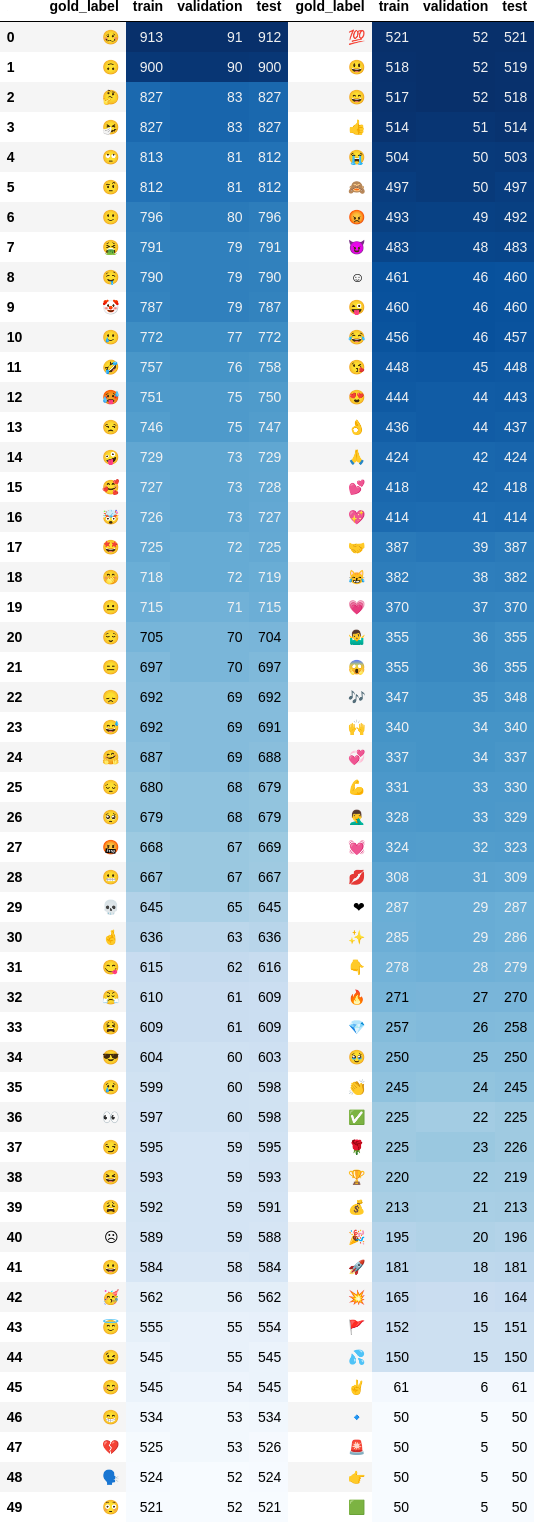
\includegraphics[scale=0.4]{../figures/super-tweeteval/emojis_dist.png}
% \caption{Emojis distribution for each split.}
% \label{appendix:SuperTweetEval-emojis-distribution}
% \end{figure*}


% First half
\begin{figure*}[!t]
\centering
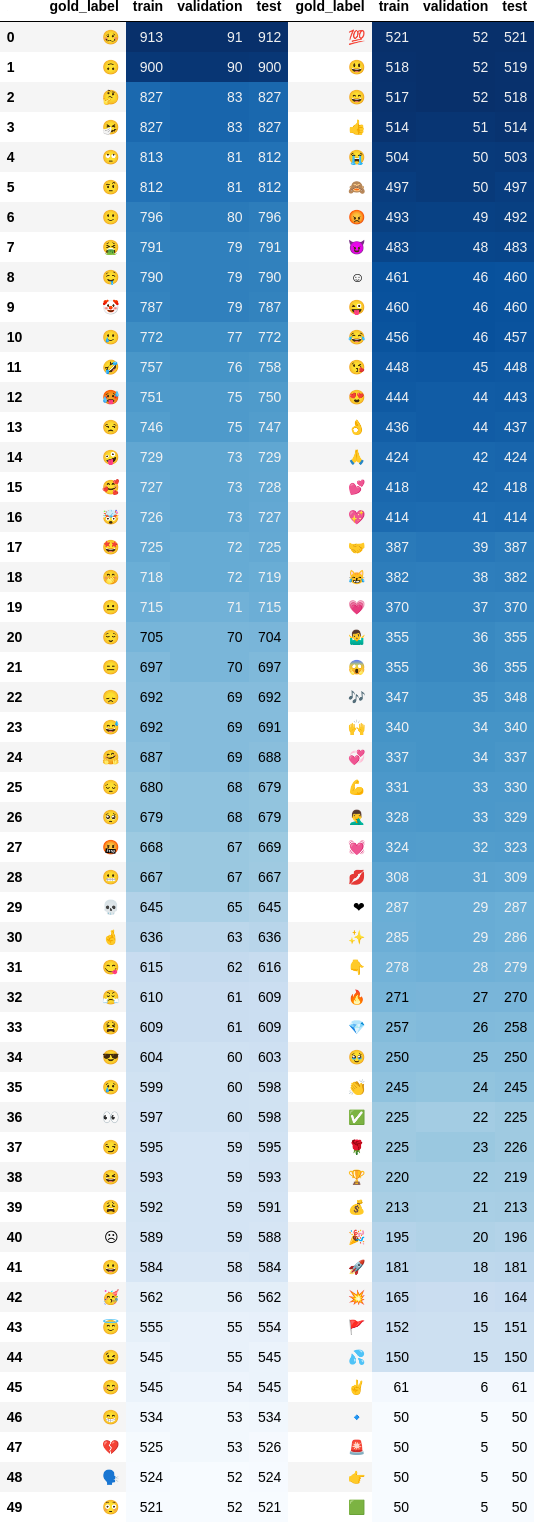
\includegraphics[scale=0.65, trim=0 740 0 0, clip]{../figures/super-tweeteval/emojis_dist.png}
\caption{Emojis distribution for each split (Part 1).}
\label{appendix:fig:super-tweeteval-emojis-dist-2}
\end{figure*}


% Second half
\begin{figure*}[!t]
\centering
{\setlength{\tabcolsep}{9pt}  % spacing between columns
\tiny
\begin{tabular}{@{}l@{\hspace{50pt}}c@{\hspace{8pt}}c@{\hspace{15pt}}c@{\hspace{20pt}}%
                l@{\hspace{30pt}}c@{\hspace{8pt}}c@{\hspace{8pt}}c@{}}
\textbf{gold\_label} & \textbf{train} & \textbf{validation} & \textbf{test} &
\textbf{gold\_label} & \textbf{train} & \textbf{validation} & \textbf{test} \\
\end{tabular}
}
\vspace{2pt} % small gap

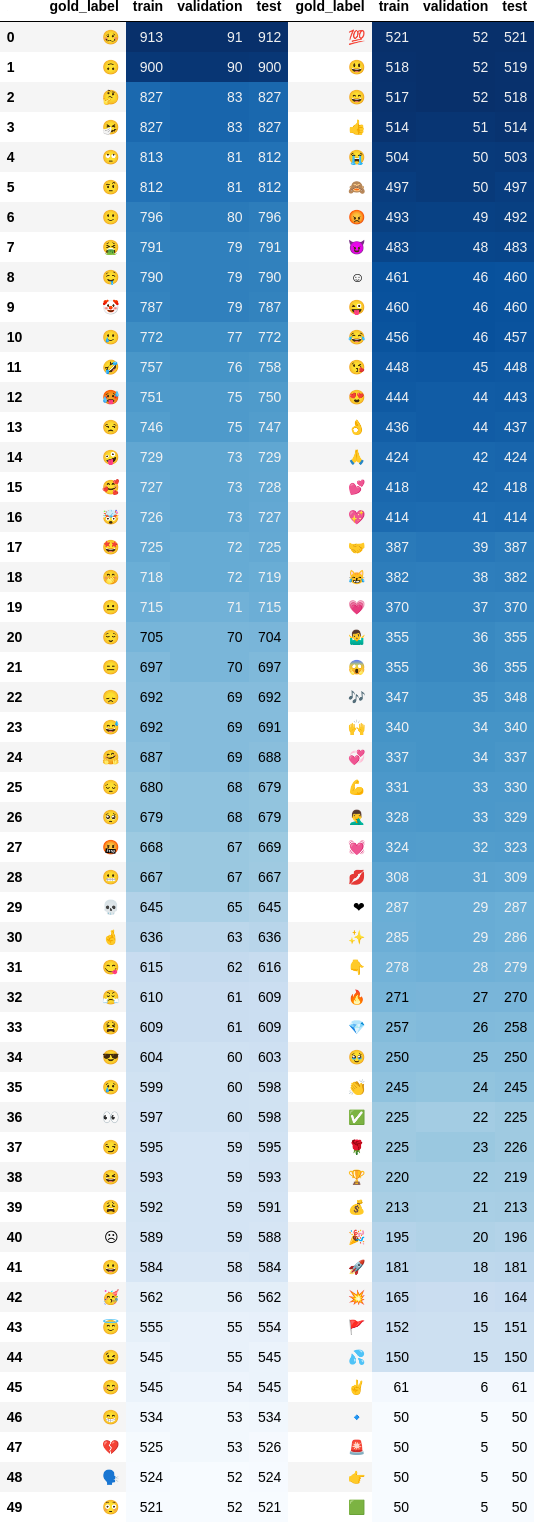
\includegraphics[scale=0.65, trim=0 0 0 740, clip]{../figures/super-tweeteval/emojis_dist.png}
\caption{Emojis distribution for each split (Part 2).}
\label{appendix:fig:super-tweeteval-emojis-dist-1}
\end{figure*}




\clearpage


\section{Politics and virality}\label{appendix:Politics}
\subsection{Data Collection}
Table \ref{tab:Politics-tweets_collected} displays the number of tweets collected from each parliament for the main time period studied, January to December 2021.

Table \ref{tab:Politics-control_stats_devolved} displays text statistics extracted from tweets of the devolved parliaments of N.Ireland, Scotland, Wales, Catalonia and Basque country. The percentage of tweets that include emojis, hashtags, mentions, and URLs as well as the percentage of upper case characters are displayed. In general, the devolved parliaments seem to follow a similar trend to their respective main bodies (Section \ref{sec:data_2021}, Table \ref{tab:control_stats}).



\begin{table*}[ht]
\begin{adjustbox}{width=\textwidth,center}
\begin{tabular}{|l|l|l|l|l|l|l|l|l|l|l|l|l|l|}
\hline
             & Jan & Feb & Mar & Apr & May   & Jun  & Jul  & Aug & Sep & Oct & Nov & Dec & \textbf{Total} \\ \hline
UK          & 47,296 & 47,606 & 38,965 & 29,336 & 34,215 & 31,081 & 31,970 & 22,044 & 27,509 & 29,557 & 31,330 & 29,026 & 399,935 \\ \hline
-Scotland  & 11,282 & 13,175 & 8,988  & 6,622  & 7,890  & 5,600  & 3,856  & 5,295  & 6,285  & 5,301  & 6,427  & 6,241  & 86,962  \\ \hline
-Wales     & 5,381  & 5,462  & 3,903  & 3,386  & 3,874  & 3,013  & 3,191  & 2,393  & 2,864  & 2,826  & 3,410  & 3,084  & 42,787  \\ \hline
-N.Ireland & 5,945  & 6,788  & 5,640  & 4,579  & 5,127  & 6,138  & 4,798  & 3,484  & 4,947  & 4,505  & 4,452  & 5,391  & 61,794  \\ \hline
Spain        & 20,119   & 25,343    & 18,407 & 18,073 & 16,938 & 16,167 & 14,732 & 11,595  & 15,376     & 14,753   & 13,823    & 13,175    & 198,501         \\ \hline
-Catalonia & 9,512  & 8,386  & 6,463  & 5,537  & 6,389  & 6,030  & 6,047  & 3,729  & 5,940  & 5,856  & 5,376  & 5,255  & 74,520  \\ \hline
-Basque    & 2,103  & 2,299  & 1,478  & 1,287  & 1,230  & 989   & 685   & 843   & 1,040  & 1,118  & 1,161  & 1,091  & 15,324  \\ \hline
Greece      & 7,234  & 9,298  & 7,421  & 7,136  & 6,345  & 6,140  & 6,239  & 4,300  & 6,060  & 5,458  & 5,941  & 5,083  & 76,655  \\ \hline
\textbf{ALL} & 108,872  & 118,357   & 91,265 & 75,956 & 82,008 & 75,158 & 71,518 & 53,683  & 70,021     & 69,374   & 71,920    & 68,346    &    956,478            \\ \hline
\end{tabular}
\end{adjustbox}
\caption{Number of MP tweets collected through 2021.}
\label{tab:Politics-tweets_collected}
\end{table*}


\begin{table}[ht]
    \centering
    \begin{tabular}{lccccc}
    \textbf{Country} & \textbf{\#} & \textbf{@} & \textbf{emoji} & \textbf{url} & \textbf{up/low} \\ \hline
    N.Ireland               & 0.04        & 0.39       & 0.25           & 0.45         & 0.11            \\ \hline
    Scotland            & 0.04        & 0.30       & 0.29           & 0.54         & 0.11            \\ \hline
    Wales           & 0.04        & 0.26       & 0.31           & 0.59         & 0.12            \\ \hline
    Catalonia           & 0.07        & 0.40       & 0.33           & 0.69         & 0.11            \\ \hline
    Basque           & 0.05        & 0.33      & 0.27           & 0.63         & 0.09            \\ \hline
    \textbf{Overall} & 0.05        & 0.34       & 0.29           & 0.58         & 0.11           
    \end{tabular}
    \caption{Percentage of tweets that include  hashtags (\#), mentions (@), emojis, and URLs in \textit{2021 Devolved Dataset}. The upper to low case ratio (upp/low) average of tweets texts is also reported.}
    \label{tab:Politics-control_stats_devolved}
\end{table}

\subsection{Extended classification results}
Table \ref{tab:Politics-f1_averages} displays the macro average F1 scores along with the average F1 scores of positive and negative classes (F1\textsuperscript{PN}) for all the experiments performed. The experiments were performed by using both a cross-validation setting (CV) and a train/test split approach. For the train/test approach the set of tweets that was annotated by all coders was used (approximately 100 tweets for each language) while the rest of the data was used for training (approximately 900 tweet for each language) (Section \ref{sec:annotation}). The results indicate the \textit{XLM-T-Sent-multi} performs consistently in both the CV and train/test settings and achieves satisfactory performance particularly for Spanish. 

% RTR 
Finally, our results demonstrate the importance that a specialised corpus can have when training the models. In particular, when looking at the $F1$ scores for the `CV' setting the models display an increased performance when trained further with the `In' domain, labelled data collected (Section \ref{sec:annotation}). The performance of `XLM-T-Sent', `TweetEval-Sent' and `Bertweet-Sent' models is increased (or at worst stays the same), across all languages tested when the `In' domain data are added to their training corpus. 
% RTR 

\begin{table*}[hbp!]
\begin{adjustbox}{width=\textwidth,center}
\begin{tabular}{|l|l|l|c|c|c|c|c|c|c|c|c|c|c|c|c|c|}
\hline
\multirow{3}{*}{Type} & \multirow{3}{*}{Model} & \multirow{3}{*}{\begin{tabular}[c]{@{}l@{}}Train \\ Lang\end{tabular}} & \multicolumn{2}{c|}{\multirow{2}{*}{Train domain}} & \multicolumn{4}{c|}{United Kingdom} & \multicolumn{4}{c|}{Spain} & \multicolumn{4}{c|}{Greece} \\ \cline{6-17} 
 &  &  & \multicolumn{2}{c|}{} & \multicolumn{2}{c|}{F1} & \multicolumn{2}{c|}{F1\textsuperscript{PN}} & \multicolumn{2}{c|}{F1} & \multicolumn{2}{c|}{F1\textsuperscript{PN}} & \multicolumn{2}{c|}{F1} & \multicolumn{2}{c|}{F1\textsuperscript{PN}} \\ \cline{4-17} 
 &  &  & Out & In & CV & split & CV & split & CV & split & CV & split & CV & split & CV & split \\ \hline
\multirow{10}{*}{\rot{Multilingual}} & \multirow{3}{*}{XLM-T} & Mono &  & \checkmark & 70 & 72 & 78 & 75 & 67 & 66 & 80 & 80 & 74 & 76 & 73 & \textbf{74} \\ \cline{3-17} 
 &  & Mono & \checkmark & \checkmark & 74 & 65 & 80 & 76 & 70 & 76 & 80 & 81 & 75 & 66 & 73 & 61 \\ \cline{3-17} 
 &  & Multi &  & \checkmark & 75 & 67 & 81 & 77 & \textbf{72} & 78 & 80 & 84 & 76 & \textbf{77} & 75 & 75 \\ \cline{2-17} 
 & \multirow{3}{*}{XLM-T-Sent} & Mono & \checkmark &  & 72 & 72 & 78 & 79 & 68 & 71 & 77 & 82 & 65 & 69 & 64 & 68 \\ \cline{3-17} 
 &  & Mono & \checkmark & \checkmark & 74 & 67 & 80 & 74 & 70 & 70 & \textbf{81} & 78 & 77 & 76 & 75 & \textbf{74} \\ \cline{3-17} 
 &  & Multi & \checkmark & \checkmark & 74 & 68 & 80 & 75 & 70 & \textbf{79} & \textbf{81} & \textbf{87} & 76 & 70 & 77 & 70 \\ \cline{2-17} 
 & \multirow{4}{*}{XLM-R} & Mono &  & \checkmark & 69 & 72 & 77 & 75 & 60 & 65 & 75 & 80 & 74 & 75 & 73 & 73 \\ \cline{3-17} 
 &  & Mono & \checkmark & \checkmark & 70 & 67 & 74 & 74 & 66 & 65 & 80 & 78 & 74 & 74 & 73 & 70 \\ \cline{3-17} 
 &  & Multi &  & \checkmark & 74 & 66 & 80 & 73 & 69 & 70 & 80 & 80 & \textbf{78} & 72 & \textbf{78} & 70 \\ \cline{3-17} 
 &  & Multi & \checkmark & \checkmark & 70 & 57 & 78 & 67 & 67 & 70 & 76 & 80 & 76 & 72 & 76 & 72 \\ \hline
\multirow{6}{*}{\rot{Monolingual}} & \multirow{2}{*}{RoBERTa-Base} & Mono &  & \checkmark & 68 & 73 & 78 & 77 & 64 & 70 & 78 & 86 & 56 & 57 & 50 & 52 \\ \cline{3-17} 
 &  & Mono & \checkmark & \checkmark & 75 & 70 & 80 & 75 & 70 & 78 & 80 & \textbf{87} & 56 & 62 & 49 & 58 \\ \cline{2-17} 
 & \multirow{2}{*}{TweetEval-Sent} & Mono & \checkmark &  & 73 & 72 & 80 & 79 & \multicolumn{8}{c|}{\multirow{4}{*}{}} \\ \cline{3-9}
 &  & Mono & \checkmark & \checkmark & 76 & 67 & 81 & 74 & \multicolumn{8}{c|}{} \\ \cline{2-9}
 & \multirow{2}{*}{Bertweet-Sent} & Mono & \checkmark &  & 77 & \textbf{76} & \textbf{83} & \textbf{83} & \multicolumn{8}{c|}{} \\ \cline{3-9}
 &  & Mono & \checkmark & \checkmark & \textbf{78} & 75 & 82 & 78 & \multicolumn{8}{c|}{} \\ \hline
- & \multirow{2}{*}{SVM} & Mono &  & \checkmark &  33 &  36 & 50 & 47 & 40 & 40  & 60 & 61 & 60 & 63 & 56 & 60 \\ \cline{1-1}  \cline{3-17} 
- &  & Mono & \checkmark & \checkmark &  47 & 47 & 61 & 57 & 42 & 38 & 58 & 57 & 52 & 55 &  44 &  51 \\ \hline
- &  \multirow{2}{*}{LSTM} & Mono  &  & \checkmark & 52  & 48 &  66 & 55 & 51 & 48 & 60 & 61 & 59 & 62 & 56 &  61\\ \cline{1-1} \cline{3-17} 
- & & Mono & \checkmark & \checkmark & 58 & 55 & 67 & 63 & 49  & 42  & 60 & 56 &  59 &60  & 57 & 59 \\ \hline
- & VADER &  &  &  & 55 & 47 & 64  & 61  & 54 & 57 & 63 & 66 & 57  & 51 & 58 & 53  \\ \hline
- & Baseline &  &  &  & 22 & 22 & 33 & 33 & 20 & 21 & 30 & 32 & 17 & 20 & 27 & 30 \\ \hline
\end{tabular}
\end{adjustbox}
\caption{Average F1 scores along with the average of F1 scores of positive and negative classes (F1\textsuperscript{PN}) when trained/evaluated with cross-validation (CV) and on the $\sim$900/100 train/test split. The results displayed are the averages of three runs. Training domain indicates the data used for training the models. `In' domain indicates models trained on the labelled data collected (Section \ref{sec:annotation}), `Out' indicates the model has been finetuned on other sentiment analysis datasets (see Section \ref{sec:expsetting}). Finally, `Mono' indicates that the model was trained with data from only one language, while `Multi' shows models that were trained with data from all available languages.}
\label{tab:Politics-f1_averages}
\end{table*}



\subsection{Extended regression results}
Table \ref{tab:Politics-poisson_results} displays the results (coefficients) of the Poisson and zero inflated Poisson regression models while using the retweet count as a dependent variable. Similarly to the \textit{NBR} models used (Section \ref{sec:sentvir}: \textit{Regression Analysis}) both Poisson models indicate that the existence of negative sentiment influences the retweet count greatly than that of positive sentiment.

\begin{table*}[hbp!]
\centering
\begin{tabular}{|l|c|c|c|c|}
\hline
\textbf{variable} & \textbf{Overall} & \textbf{UK} & \textbf{Spain} & \textbf{Greece} \\ \hline
const             & 72.8914*         & 75.9854*    & 96.6305*       & 96.6305*        \\ \hline
emojis            & -5.1085*         & -7.9482*    & -9.7004*       & -9.7004*        \\ \hline
has\_url          & -1.3613          & -17.524*    & 26.56*         & 26.56*          \\ \hline
hashtags          & -20.0335*        & -7.811*     & -41.0476*      & -41.0476*       \\ \hline
mentions          & -41.0511*        & -40.4977*   & -63.0461*      & -63.0461*       \\ \hline
max\_score        & -43.16*          & -42.5478*   & -39.615*       & -39.615*        \\ \hline
\end{tabular}
\caption{Coefficients for the OLS model when using tweets from the combined 2021 UK, Spain, Greece parliaments and for each individual parliament. Dependent variable is the retweet count while XLM-T's softmax scores (negative and positive sentiment) are utilised (sent score) as independent variables.  $*$ indicates p-value $< 0.05$ }
\label{tab:Politics-ols_results}
\end{table*}

Table \ref{tab:Politics-ols_results} shows the coefficients for each predictor when using the softmax scores of the positive and negative sentiments of the \textit{XLM-T} model instead of the final label. For each entry the highest absolute softmax score is considered and is assigned positive or negative sign based on the sentiment. The results indicate, i.e., negative coefficient, that the "more" negative a tweet the more is retweeted.



\begin{table*}[hbp!]
\begin{adjustbox}{width=\textwidth,center}
\begin{tabular}{|l|cc|cc|cc|cc|}
\hline
\multirow{2}{*}{\textbf{variable}} &
  \multicolumn{2}{c|}{\textbf{Overall}} &
  \multicolumn{2}{c|}{\textbf{UK}} &
  \multicolumn{2}{c|}{\textbf{Spain}} &
  \multicolumn{2}{c|}{\textbf{Greece}} \\ \cline{2-9} 
 &
  \multicolumn{1}{c|}{\textbf{Poisson}} &
  \textbf{zero Poisson} &
  \multicolumn{1}{c|}{\textbf{Poisson}} &
  \textbf{zero Poisson} &
  \multicolumn{1}{c|}{\textbf{Poisson}} &
  \textbf{zero Poisson} &
  \multicolumn{1}{c|}{\textbf{Poisson}} &
  \textbf{zero Poisson} \\ \hline
const &
  \multicolumn{1}{c|}{3.4035*} &
  4.0809* &
  \multicolumn{1}{c|}{3.7006*} &
  4.4486* &
  \multicolumn{1}{c|}{3.61*} &
  4.1586* &
  \multicolumn{1}{c|}{2.3372*} &
  2.8278* \\ \hline
emojis &
  \multicolumn{1}{c|}{-0.193*} &
  -0.1769* &
  \multicolumn{1}{c|}{-0.3277*} &
  -0.2978* &
  \multicolumn{1}{c|}{-0.2114*} &
  -0.1946* &
  \multicolumn{1}{c|}{-0.3298*} &
  -0.3639* \\ \hline
has\_url &
  \multicolumn{1}{c|}{0.013*} &
  -0.3695* &
  \multicolumn{1}{c|}{-0.3798*} &
  -0.8422* &
  \multicolumn{1}{c|}{0.41*} &
  0.0827* &
  \multicolumn{1}{c|}{-0.1871*} &
  -0.305* \\ \hline
hashtags &
  \multicolumn{1}{c|}{-0.5219*} &
  -0.6281* &
  \multicolumn{1}{c|}{-0.4001*} &
  -0.5168* &
  \multicolumn{1}{c|}{-0.5878*} &
  -0.6266* &
  \multicolumn{1}{c|}{-0.3372*} &
  -0.41* \\ \hline
mentions &
  \multicolumn{1}{c|}{-1.0543*} &
  -0.7944* &
  \multicolumn{1}{c|}{-1.4615*} &
  -0.8382* &
  \multicolumn{1}{c|}{-0.929*} &
  -0.8291* &
  \multicolumn{1}{c|}{-0.9082*} &
  -0.7696* \\ \hline
neg &
  \multicolumn{1}{c|}{1.4129*} &
  1.1709* &
  \multicolumn{1}{c|}{1.3014*} &
  1.0566* &
  \multicolumn{1}{c|}{1.1818*} &
  1.0028* &
  \multicolumn{1}{c|}{0.9232*} &
  0.6859* \\ \hline
pos &
  \multicolumn{1}{c|}{0.2295*} &
  0.1629* &
  \multicolumn{1}{c|}{-0.1486*} &
  -0.1855* &
  \multicolumn{1}{c|}{0.5513*} &
  0.4503* &
  \multicolumn{1}{c|}{0.3229*} &
  0.2315* \\ \hline
\end{tabular}
\end{adjustbox}
\caption{Coefficients for the Poisson Regression and zero inflated Poisson Regression when using tweets from the combined 2021 UK, Spain, Greece parliaments and for each individual parliament. Dependent variable is the retweet count while the independent variables \textit{neg} and \textit{pos} indicate the sentiment according to XLM-T results. $*$ indicates p-value $< 0.05$ }.
\label{tab:Politics-poisson_results}
\end{table*}




\section{Fake news spreaders}
\subsection{Computational Resources}
\label{sec:appendix-models}
An \textit{NVIDIA GeForce RTX 4090} GPU was utilised for the experiments conducted:
\begin{itemize}
    \item 18 hours for the inference process of (sentiment, emotion, topic) on the \textit{MBFC}, \textit{FNN}, and \textit{Verified} datasets.
    \item 6 hours for the training of the Longformer model (Section \textit{Spreader Detection Analysis}.
\end{itemize}
 % with a total utilisation of 6 hours.

\subsection{Model Categories}
\subsubsection{Emotion Categories}
\label{sec:emotion-list}
The \textit{twitter-roberta-base-emotion-multilabel} model classifies each entry in one or more of the following classes:
\textit{anger, anticipation, disgust, fear, joy, love, optimism, pessimism, sadness, surprise, trust}.

\subsubsection{Hate Speech Categories.}
\label{sec:hate-list}
The \textit{twitter-roberta-base-hate-multiclass}  model classifies each entry in one of the following classes: \textit{not\_hate, sexism, racism, religion, other, sexual\_orientation, disability}

\subsubsection{Topic Classification Categories}
\label{sec:topic-list}
The \textit{tweet-topic-21-multi} model assigns each tweet one or more topics from the following list: 
\textit{arts\_\&\_culture, business\_\&\_entrepreneurs, celebrity\_\&\_pop\_culture, diaries\_\&\_daily\_life, family, fashion\_\&\_style, film\_tv\_\&\_video, fitness\_\&\_health, food\_\&\_dining, gaming, learning\_\&\_educational, music, news\_\&\_social\_concern, other\_hobbies, relationships, science\_\&\_technology, sports, travel\_\&\_adventure, youth\_\&\_student\_life}


\subsection{Spreader Detection: \textit{XGB}}
\label{appendix:xgb}


Table \ref{tab:xgb-extra} highlights the performance of each feature set, with the 'text and sentiment (text-s)' combination achieving the highest F1 score of 75 and accuracy of 76, suggesting it is the most effective combination for this analysis.


\begin{table}[]
\centering
\begin{tabular}{|l|c|c|}
\hline
\textbf{Features} & \textbf{F1} & \textbf{Accuracy} \\ \hline
text     & 74          & 74                \\ \hline
text-s   & \textbf{75}          & \textbf{76}                \\ \hline
text-e   & 72          & 72                \\ \hline
text-t   & 69          & 69                \\ \hline
text-st  & 71          & 71                \\ \hline
text-se  & 73          & 73                \\ \hline
text-et  & 68          & 69                \\ \hline
text-set & 72          & 72                \\ \hline
\end{tabular}

\caption{Comparative results of F1 scores and accuracy for various feature combinations using the XGB classifier on the \textit{PAN} dataset. \textit{s: sentiment, e: emotion, t: topic}}\label{tab:xgb-extra}
\end{table}


Figures \ref{fig:hate-distribution-xgb}, \ref{fig:sentiment-distribution-xgb}, and \ref{fig:emotion-distribution-xgb} illustrate that the discrepancies in the distribution of the examined features, sentiment, emotion and hate speech respectively\footnote{Results related to the topic distribution can be found in Appendix \ref{appendix:xgb}.}, between the XGB model's predictions and the \textit{PAN} dataset are negligible, indicating that they exhibit comparable trends.


\begin{figure*}
  \begin{subfigure}{0.5\textwidth}
    \centering
    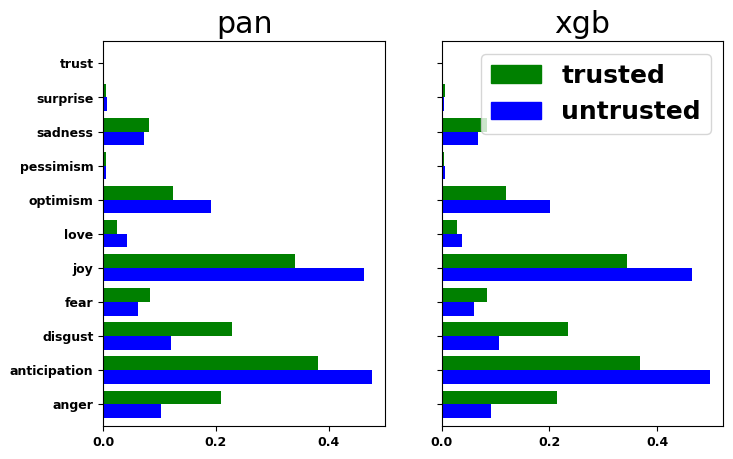
\includegraphics[width=\linewidth]{../figures/spreaders/pan-xgb-emotion.png}
    \caption{Emotion distribution comparison between the \textit{PAN} dataset and the predictions from the \textit{XGB} model.}
    \label{fig:emotion-distribution-xgb}
  \end{subfigure}%
  \begin{subfigure}{0.5\textwidth}
    \centering
    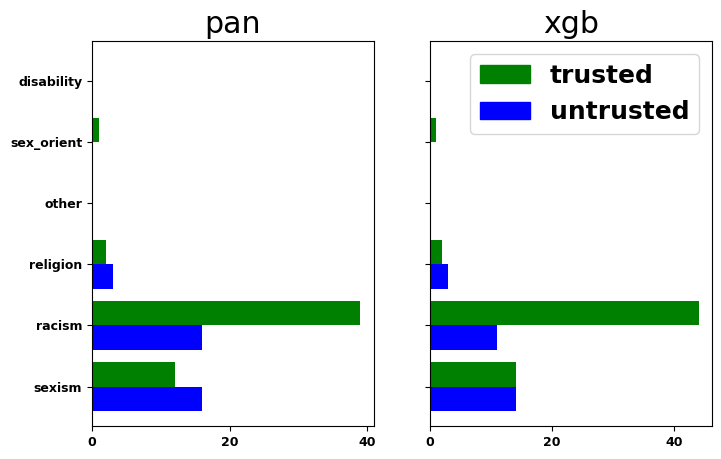
\includegraphics[width=\linewidth]{../figures/spreaders/pan-xgb-hate.png}
    \caption{Hate speech distribution comparison between the \textit{PAN} dataset and the predictions from the \textit{XGB} model.}
    \label{fig:hate-distribution-xgb}
  \end{subfigure}
  \caption{Emotion \& Hate speech results for \textit{PAN} dataset and \textit{XGB} model.}
\end{figure*}


\begin{figure*}[!ht]
\centering
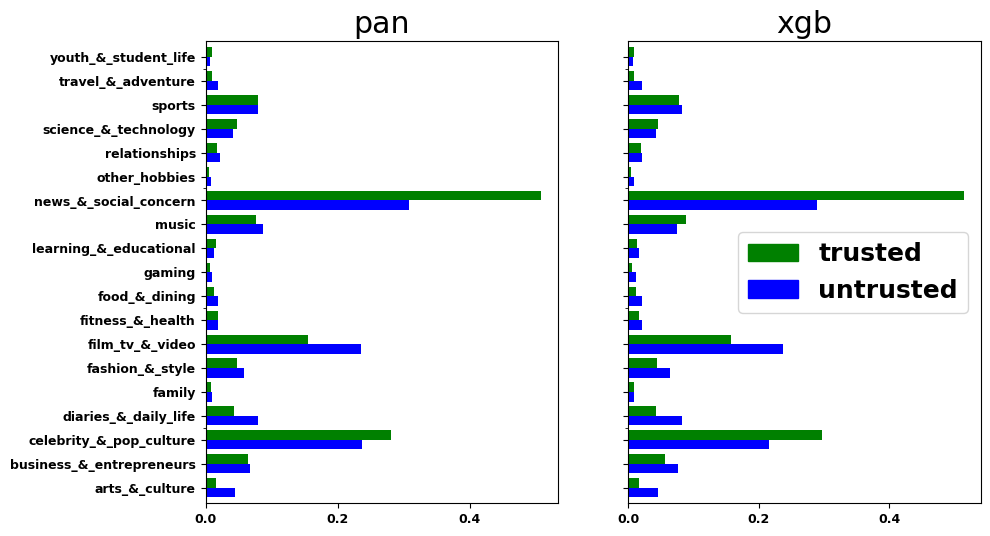
\includegraphics[scale=0.45]{../figures/spreaders/pan-xgb-topics.png}
\caption{Topic distribution comparison between the \textit{PAN} dataset and the predictions from the \textit{XGB} model.}
\label{fig:topics-distribution-xgb}
\end{figure*}


\begin{figure}[!ht]
\begin{adjustbox}{width=\linewidth,center}
\centering
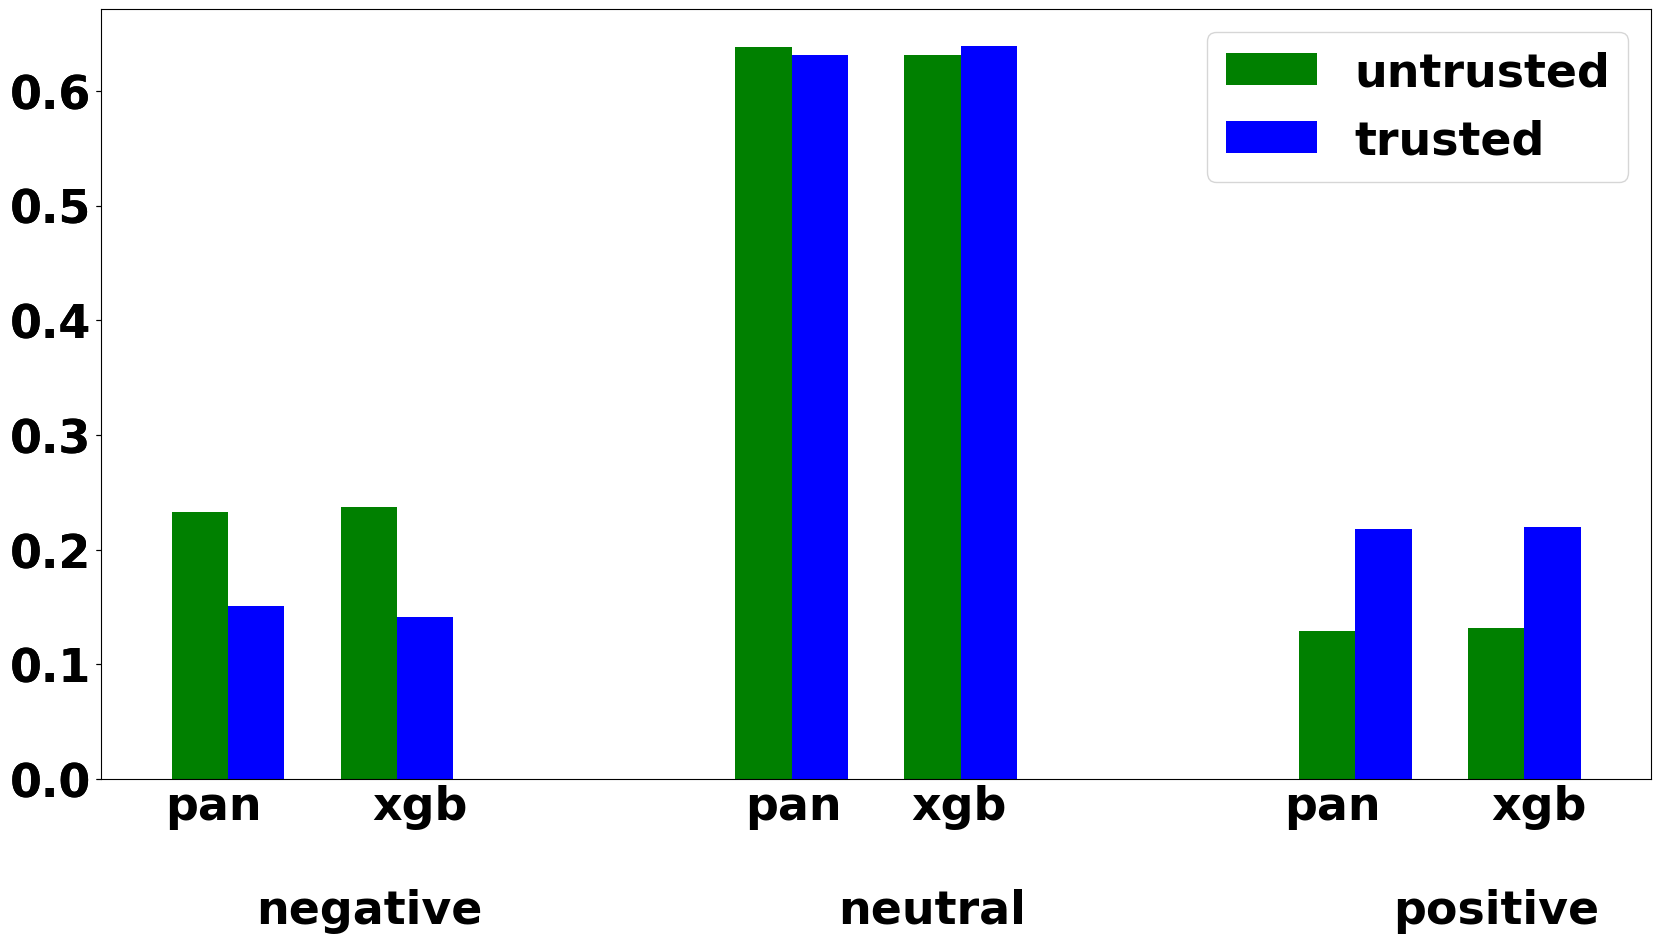
\includegraphics[scale=0.8]{../figures/spreaders/pan-xgb-sentiment.png}
\end{adjustbox}
\caption{Sentiment comparison between \textit{PAN} dataset and the \textit{XGB} models' predictions.}
\label{fig:sentiment-distribution-xgb}
\end{figure}


\clearpage


\section{Trigger points}
\subsection{Model Selection}
\subsection{Emotion Categories}
\label{sec:triggers-emotion-list}
The \textit{twitter-roberta-base-emotion-multilabel} model classifies each entry in one or more of the following classes:
\textit{anger, anticipation, disgust, fear, joy, love, optimism, pessimism, sadness, surprise, trust}.

\subsubsection{Hate Speech Categories.}
\label{sec:triggers-hate-list}
The \textit{twitter-roberta-base-hate-multiclass}  model classifies each entry in one of the following classes: \textit{not\_hate, sexism, racism, religion, other, sexual\_orientation, disability}

\subsubsection{Validation Setting}
\label{sec:validation}
Table \ref{tab:annotated_data} displays the distribution of comments in regards to emotion, sentiment and hate speech for the manually annotated dataset collected.

\begin{table}[ht]
\centering
\begin{tabular}{llll|ll}
\multicolumn{2}{c|}{Emotion}            & \multicolumn{2}{c|}{Hate Speech}       & \multicolumn{2}{c}{Sentiment}         \\ \hline
no emotion & \multicolumn{1}{l|}{29} & not hate     & 88     & negative     & 56    \\
anger      & \multicolumn{1}{l|}{26} & sexism       & 7      & neutral      & 37    \\
disgust    & \multicolumn{1}{l|}{23} & racism       & 3      & positive     & 7     \\
pessimism    & \multicolumn{1}{l|}{19} & other                & 2               & \multicolumn{2}{l}{\multirow{6}{*}{}} \\
anticipation & \multicolumn{1}{l|}{15} & \multicolumn{2}{l|}{\multirow{5}{*}{}} & \multicolumn{2}{l}{}                  \\
sadness    & \multicolumn{1}{l|}{9}  & \multicolumn{2}{l|}{} & \multicolumn{2}{l}{} \\
surprise   & \multicolumn{1}{l|}{5}  & \multicolumn{2}{l|}{} & \multicolumn{2}{l}{} \\
optimism   & \multicolumn{1}{l|}{5}  & \multicolumn{2}{l|}{} & \multicolumn{2}{l}{} \\
joy        & \multicolumn{1}{l|}{2}  & \multicolumn{2}{l|}{} & \multicolumn{2}{l}{}
\end{tabular}
\caption{Distribution of comments regarding emotion, sentiment, and hate speech categories on the manually annotated dataset.}
\label{tab:annotated_data}
\end{table}

\subsubsection{Annotation Guidelines}
\label{sec:appendix_guidelines}
Below we present the guidelines presented to annotators for the Sentiment Analysis, Emtion classification, and Hate Speech detection tasks.

\subsubsection*{Sentiment Analysis}
We will show you Reddit comments that can be positive, negative, or neutral based on their sentiment. 

\noindent \textbf{Sentiment Categories}
\begin{itemize}
    \item Positive comments should be labelled: \textbf{Positive}
    \item Neutral comments should be labelled:  \textbf{Neutral}
    \item Negative comments should be labelled: \textbf{Negative}
\end{itemize}

\noindent \textbf{Examples}
\begin{itemize}
    \item ```Just finished my morning workout and feeling fantastic!  \#HealthyLiving \#FitnessGoals``` is a positive sentence.
    \item ```Stuck in traffic again!  Late for work and already stressed out. \#TrafficJam``` \#MondayBlues is a negative  sentence.
    \item Factual sentences such as ```The party was in front of the house``` are neutral  sentences.
\end{itemize}

\noindent \textbf{Notes:}
\noindent We have also added a comment column where you can share your thoughts, comments, or doubts. If you are unsure whether you should annotate the tweet as positive, negative or neutral, you may choose the label that suits it best and a comment about that in the comment column. 

\noindent  The annotation of an ironic comments depends on the context. While we acknowledge the lack of context, if you think the tweet is mocking someone (or a group of people), you should label it negative.


\subsubsection*{Emotion Classification}
You will be presented with Reddit comments and asked to select the option that best describes the text.
You may choose as many emotions as you believe are present — from 0 to 11 — based on the content and tone of the comment.


\noindent\textbf{Emotion Categories:}
\begin{itemize}
    \item \textbf{Anger} – includes annoyance, rage
    \item \textbf{Anticipation} – includes interest, vigilance
    \item \textbf{Disgust} – includes disinterest, dislike, loathing
    \item \textbf{Fear} – includes apprehension, anxiety, terror
    \item \textbf{Joy} – includes serenity, ecstasy
    \item \textbf{Love} – includes affection
    \item \textbf{Optimism} – includes hopefulness, confidence
    \item \textbf{Pessimism} – includes cynicism, no confidence
    \item \textbf{Sadness} – includes pensiveness, grief
    \item \textbf{Surprise} – includes distraction, amazement
    \item \textbf{Trust} – includes acceptance, liking, admiration
\end{itemize}


\noindent\textbf{Notes:}
\noindent If no emotion is clearly present, you may leave all options unchecked. Choose all emotions that are clearly expressed or implied in the comment. If you're unsure, use the comment column to share your reasoning or highlight ambiguity. Comments may express multiple emotions simultaneously, for example, both sadness and anger.

\subsubsection*{Hate Speech Detection}
You will be presented with Reddit comments and asked to identify whether they contain hate speech, and if so, which target group is being attacked or discriminated against.
Please choose \textbf{only one} of the following categories that best represents the nature of the content:

\noindent\textbf{Hate Speech Categories:}
\begin{itemize}
    \item \textbf{Sexism}: Content that targets or demeans people based on their gender (e.g., women, men, non-binary individuals) or reinforces harmful gender stereotypes. Example: ``Women should stay in the kitchen where they belong."
    
    \item \textbf{Racism}: Content that expresses hostility, prejudice, or dehumanization based on race, ethnicity, or national origin. Example: ``All [ethnic group] are criminals and should be deported."
    
    \item \textbf{Disability}: Content that mocks, belittles, or degrades people with physical, mental, or developmental disabilities. Example: ``You're so stupid, you must be on the spectrum."
    
    \item \textbf{Sexual Orientation}: Hate directed toward someone because of their actual or perceived sexual orientation (e.g., gay, lesbian, bisexual, etc.). Example: ``Being gay is a disease that should be cured."
    
    \item \textbf{Religion}: Disparagement, dehumanization, or threats against individuals or groups based on religious beliefs or identities. Example: ``All Muslims are terrorists."
    
    \item \textbf{Other}: Use this label for hate speech that targets a group not covered above, such as socioeconomic status, age, appearance, political affiliation, etc. Example: ``Old people are useless and should just die already."
    
    \item \textbf{Not Hate}: Use this label if the comments does not contain hate speech. Comments that are neutral or non-discriminatory.
\end{itemize}

\noindent \textbf{Notes:}
If you are unsure, select the label you think fits best and add a comment explaining your reasoning. A single post may mention multiple groups in such a case, select the one that is most explicit or harmful, and explain in the comment column.



\subsection{Extended Results}
\label{sec:appendix_counts}

Table \ref{tab:trigger_counts} presents the total number of comments and threads extracted from Reddit for each keyword, along with the corresponding time periods during which the data was collected.

Table \ref{tab:comment_count} presents the number of comments included in each experiment for both the treatment and control groups.

Figure \ref{fig:absolute_counts_overall} displays the number of comments posted before and after the introduction of each trigger point on the data collected.

Figure \ref{fig:rwanda_controv_temporal_semantic} displays the average controversiality per thread before and after the introduction of the \textit{Rwanda} trigger point in the Temporal and Contextual control settings.

Figure \ref{fig:rwanda_temporal_semantic} displays the distribution of comments posted before and after the introduction of the \textit{Rwanda} trigger point in the Temporal and Contextual control settings.

Figure \ref{fig:sentiment_space_Appendix} displays the distribution of negative comments, based on their sentiment, posted before and after the introduction of the \textit{Brexit, Feminism, Rwanda, and NHS} trigger points in the Space control setting.

Figure \ref{fig:emotion_space_vaccine} displays the distribution of comments conveying anger and those that do not before and after the introduction of the \textit{Vaccine} trigger point in the Space control setting.


\begin{table}[]
\centering
\scalebox{1}{
\begin{tabular}{l|ccc}
\textbf{}           & \textbf{Threads} & \textbf{Comments} & \textbf{Year} \\ \hline
\textbf{Rwanda}     & 0.05             & 1.87              & 2020, 2022    \\ \hline
\textbf{Brexit}     & 0.37             & 11.57             & 2020 - 2022   \\ \hline
\textbf{NHS}        & 0.34             & 6.20              & 2020 - 2022   \\ \hline
\textbf{Vaccine}    & 1.42             & 28.11             & 2019, 2022    \\ \hline
\textbf{Feminism}   & 0.94             & 17.79             & 2020 - 2022   \\ \hline
\textbf{EU}         & 0.2              & 12.4              & 2020 - 2022   \\ \hline
\textbf{Red Cross}  & 0.02             & 0.2               & 2020 - 2022   \\ \hline
\textbf{SubSaharan} & 0.08             & 1.5               & 2020, 2022    \\ \hline
\textbf{Surgery}    & 0.5              & 3.9               & 2019, 2022    \\ \hline
\textbf{Woman}      & 2.1              & 19.3              & 2020 - 2022  \\
\bottomrule
\end{tabular}}
\caption{Numbers, in millions, of threads, comments, and time period for each trigger word.}
\label{tab:trigger_counts}
\end{table}

\begin{table}[]
\centering
\begin{tabular}{l|lrr}
\multicolumn{1}{c|}{\textbf{Trigger}} & \multicolumn{1}{c}{\textbf{Experiment}} & \textbf{Treatment} & \textbf{Control} \\ \hline
\multirow{2}{*}{Feminist} & space    & \multirow{2}{*}{264,495} & 16,503,956 \\
                          & contextual &                         & 163,740   \\ \hline
\multirow{3}{*}{Rwanda}   & space    & \multirow{3}{*}{28,770}  & 668,641   \\
                          & contextual &                         & 2,587     \\
                          & temp     &                         & 5,896     \\ \hline
\multirow{2}{*}{Brexit}   & space    & \multirow{2}{*}{688,600} & 10,793,036 \\
                          & contextual &                         & 111,524   \\ \hline
\multirow{3}{*}{vaccine}  & space    & \multirow{3}{*}{348,641} & 7,685,095  \\
                          & contextual &                         & 12,986    \\
                          & temp     &                         & 11,841    \\ \hline
\multirow{2}{*}{NHS}      & space    & \multirow{2}{*}{509,458} & 5,275,917  \\
                          & contextual &                         & 1,276    
\end{tabular}
\caption{Number of comments present for each trigger in each experiment for both the treatment and control subsets.}
\label{tab:comment_count}
\end{table}

\begin{figure}[ht]
    \centering
    % Row 1
    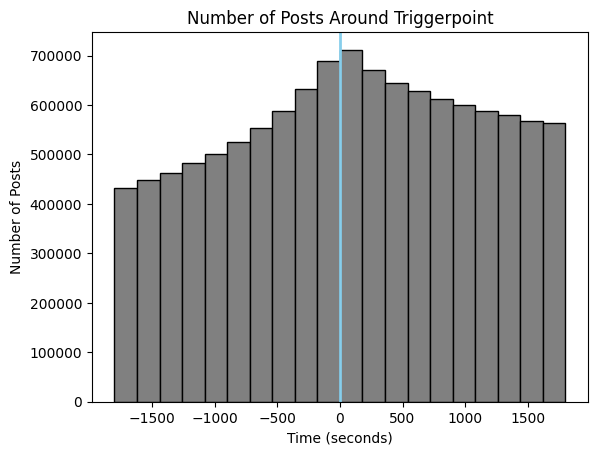
\includegraphics[width=0.49\textwidth]{../figures/triggers/counts/overall/brexit.png}
    \hfill
    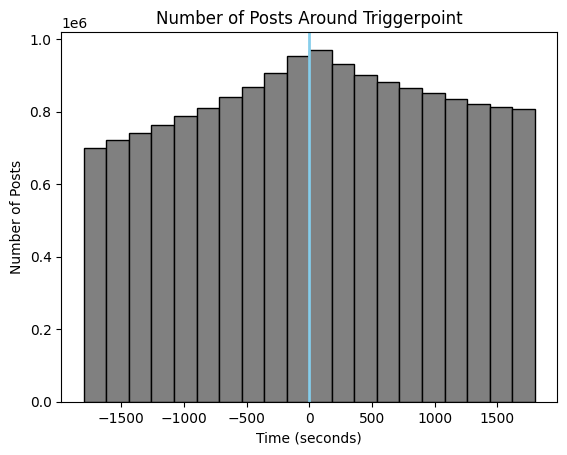
\includegraphics[width=0.49\textwidth]{../figures/triggers/counts/overall/feminism.png}
    
    % Row 2
    \vspace{1em}
    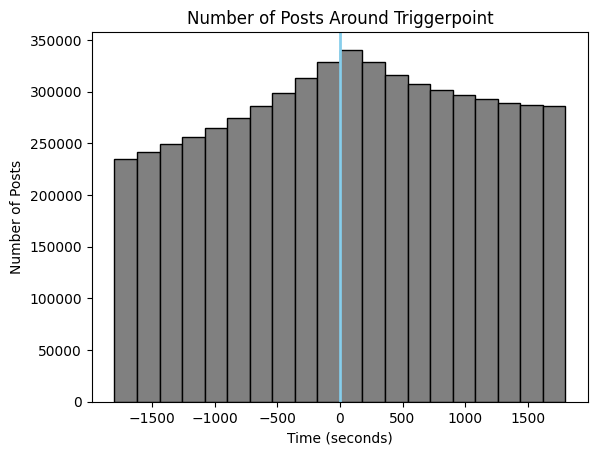
\includegraphics[width=0.49\textwidth]{../figures/triggers/counts/overall/nhs.png}
    \hfill
    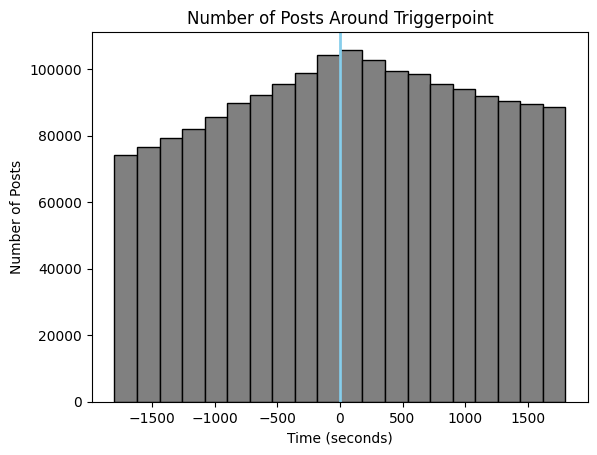
\includegraphics[width=0.49\textwidth]{../figures/triggers/counts/overall/rwanda.png}
    
    % Row 3
    \vspace{1em}
    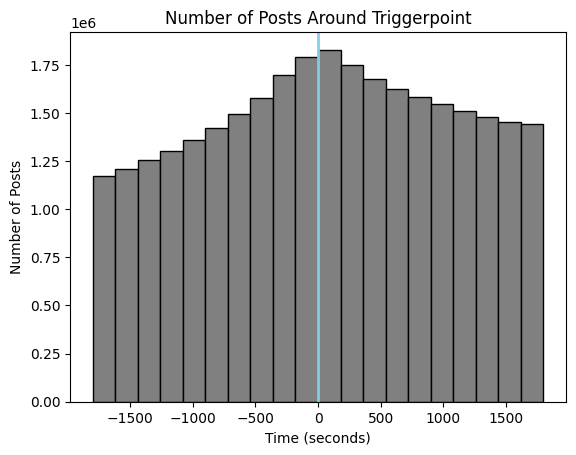
\includegraphics[width=0.49\textwidth]{../figures/triggers/counts/overall/vaccine.png}
    
    \caption{Absolute count of comments before and after each trigger point.}
    \label{fig:absolute_counts_overall}
\end{figure}



\begin{figure}[ht]
    \centering
    % First image
    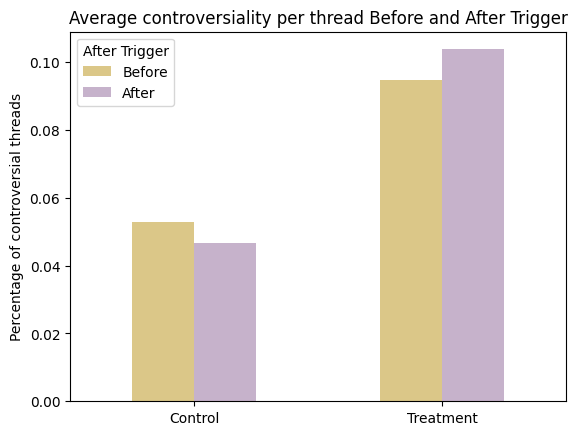
\includegraphics[width=\textwidth]{../figures/triggers/controversiality/rwanda_temporal.png}
    \vspace{1em} % vertical space
    % Second image
    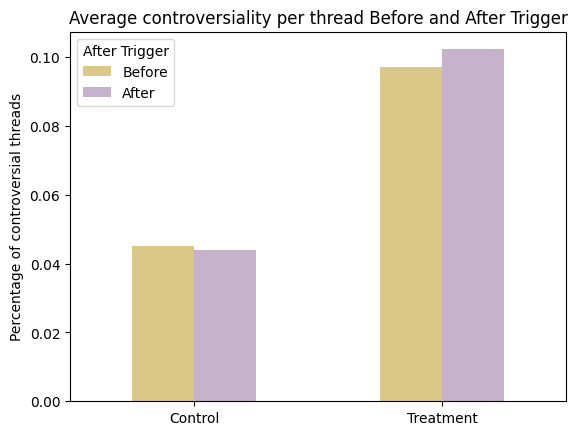
\includegraphics[width=\textwidth]{../figures/triggers/controversiality/rwanda_semantics.png}
    
    \caption{Average controversiality per thread in the Temporal and Contextual settings and their respective treatment groups, for the trigger point \textit{Rwanda}.}
    \label{fig:rwanda_controv_temporal_semantic}
\end{figure}


\begin{figure}[ht]
    \centering
    % Contextual Comparison
    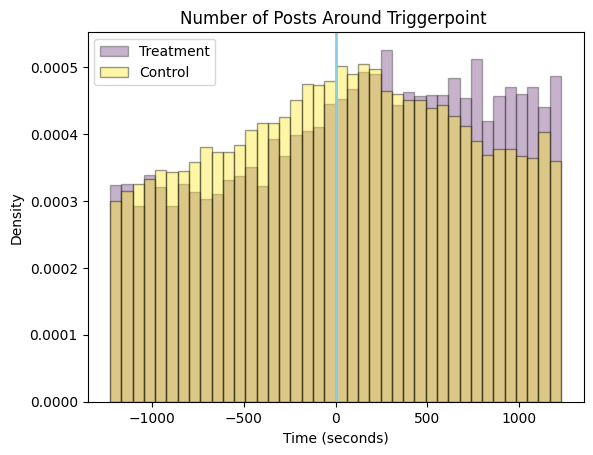
\includegraphics[width=\textwidth]{../figures/triggers/counts/counts_sem/rwanda.png}
    \vspace{1em} % space between plots
    % Temporal Comparison
    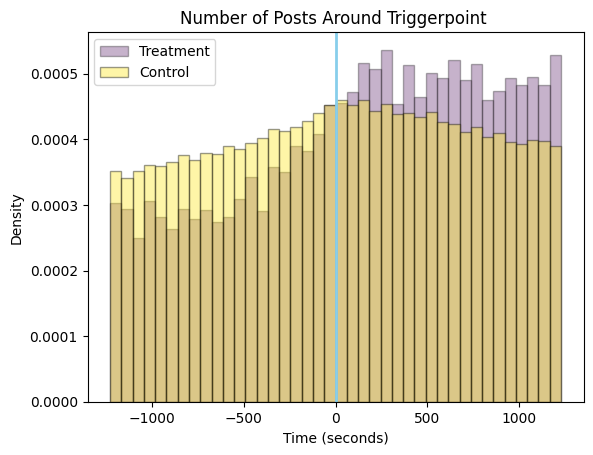
\includegraphics[width=\textwidth]{../figures/triggers/counts/counts_temp/rwanda.png}

    \caption{Rwanda Treatment and Control distributions of comments in the Contextual and Temporal settings.}
    \label{fig:rwanda_temporal_semantic}
\end{figure}


\begin{figure}[ht]
    \centering
    % Row 1
    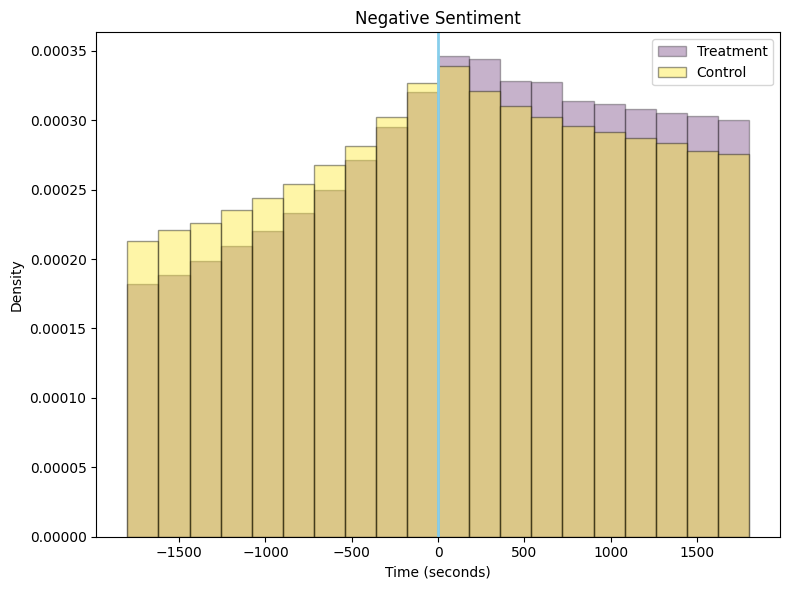
\includegraphics[width=0.75\textwidth]{../figures/triggers/sentiment/space/brexit.png}
    \vspace{1em}
    % Row 2
    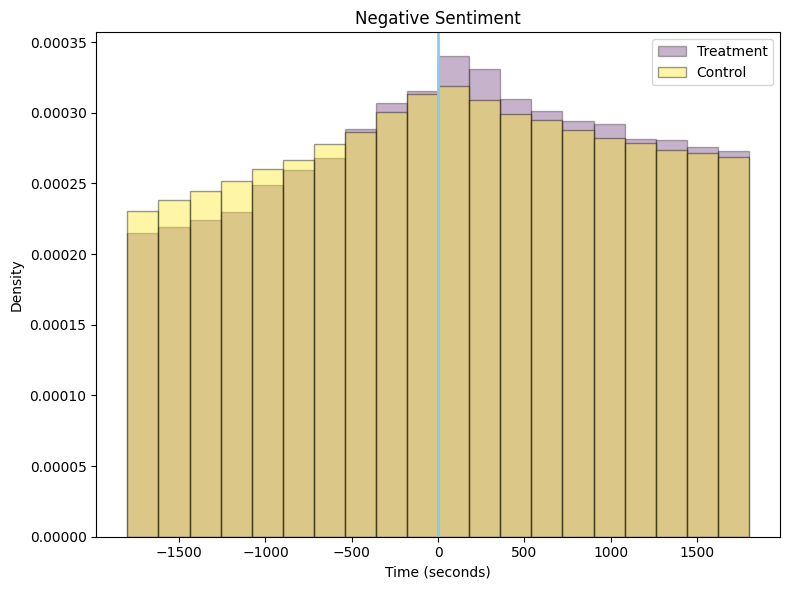
\includegraphics[width=0.75\textwidth]{../figures/triggers/sentiment/space/feminism.png}
    \vspace{1em}
    % Row 3
    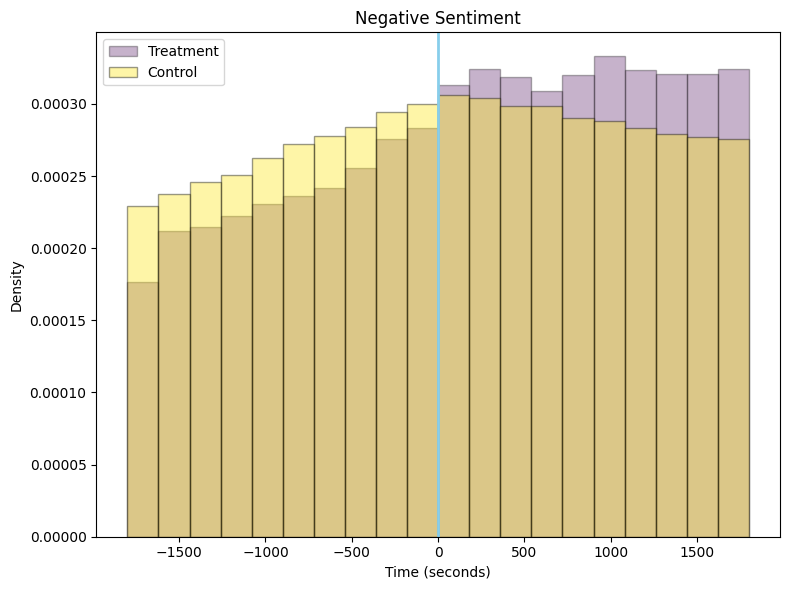
\includegraphics[width=0.49\textwidth]{../figures/triggers/sentiment/space/rwanda.png}
    \hfill
    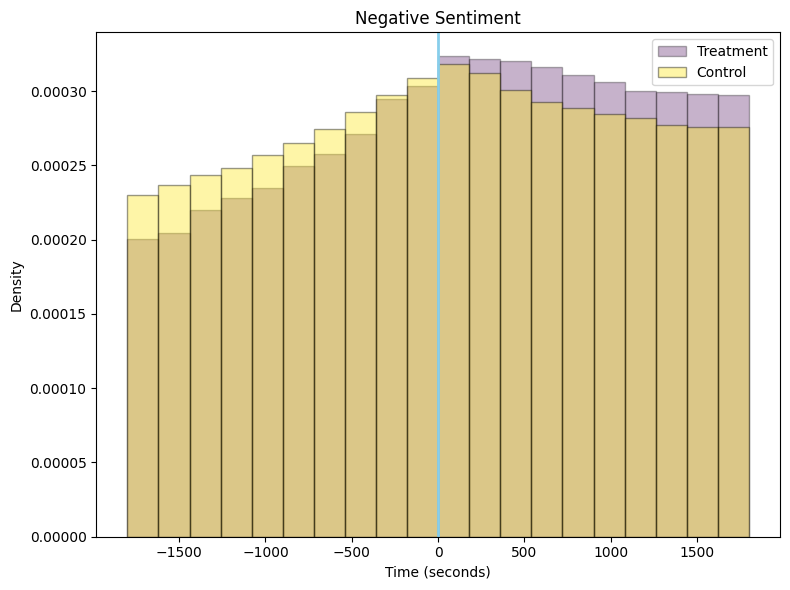
\includegraphics[width=0.49\textwidth]{../figures/triggers/sentiment/space/nhs.png}

    \caption{Distribution of negatively charged comments in the Treatment and Control (Space) groups.}
    \label{fig:sentiment_space_Appendix}
\end{figure}


\begin{figure*}
    \centering
    \resizebox{\textwidth}{!}{
    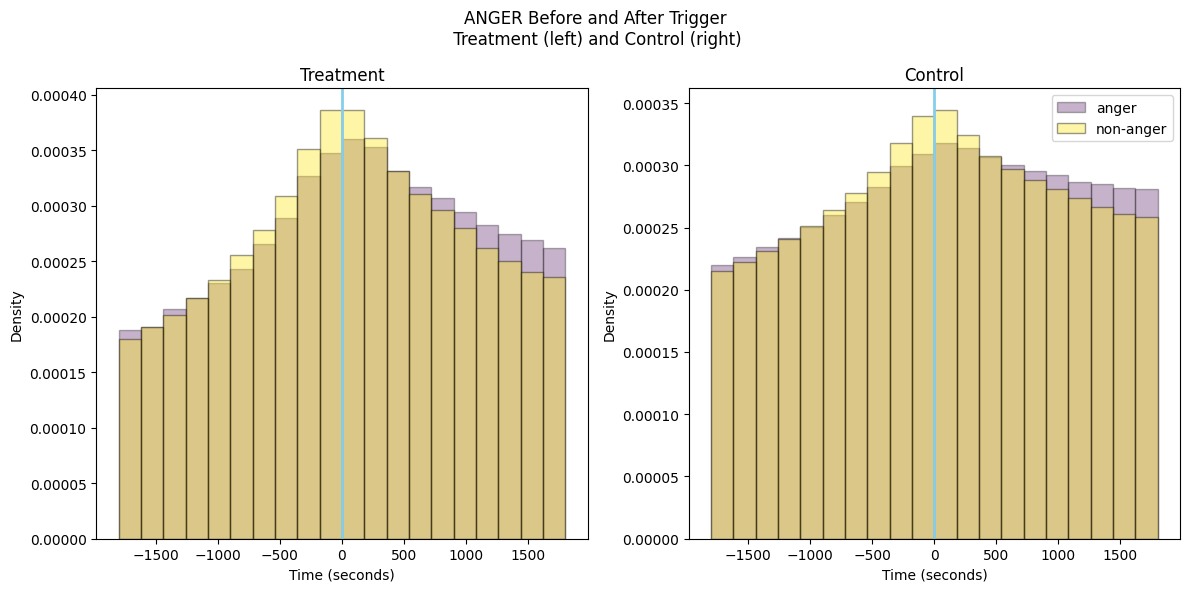
\includegraphics{../figures/triggers/emotion/space/vaccine.png}
    }
    \caption{Distribution of anger and non-anger comments for the treatment and control (space) groups of \textit{Vaccine} trigger word.}
    \label{fig:emotion_space_vaccine}
\end{figure*}


\subsection{Extended Test of Parallel Trends Assumption}
Figures \ref{fig:parallel_trends} \textit{a \& b} display the results of the Parallel Trends Assumption testing for all experiments as described in H1 and H2.


\begin{figure*}[ht]
    \centering
    \begin{subfigure}[b]{1\columnwidth}
        \centering
        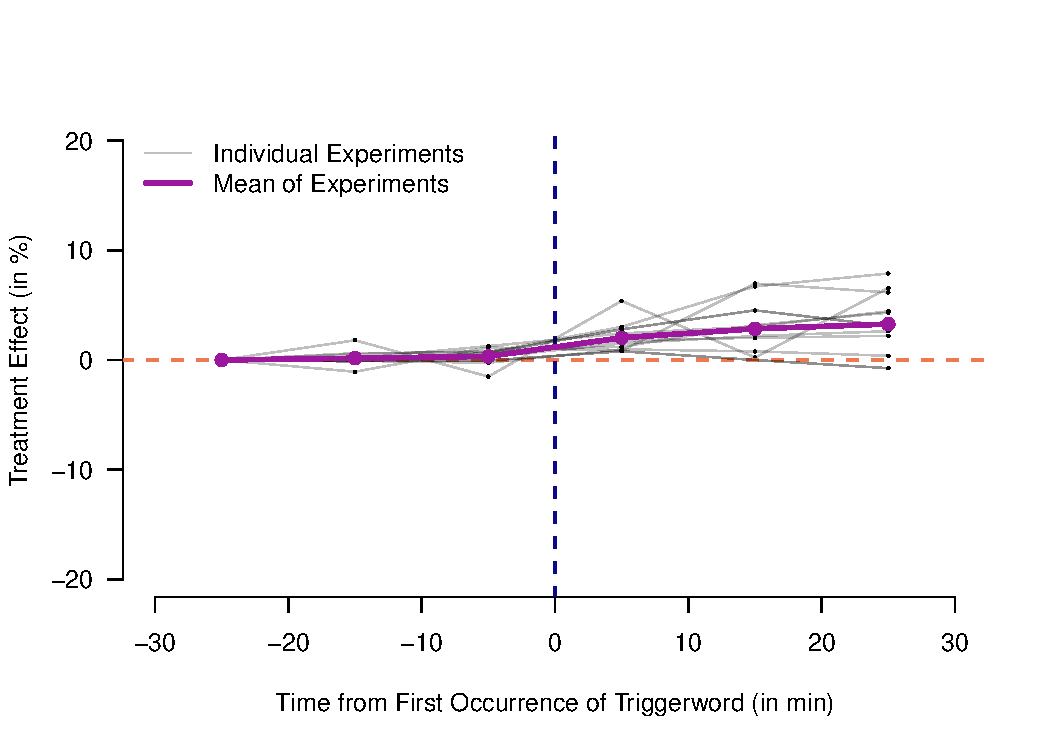
\includegraphics[width=\textwidth]{../figures/triggers/robustness_event_study_H1.pdf}
        \caption{Experiments from H1.}
        \label{fig:image5a}
    \end{subfigure}
    \hfill
    \begin{subfigure}[b]{1\columnwidth}
        \centering
        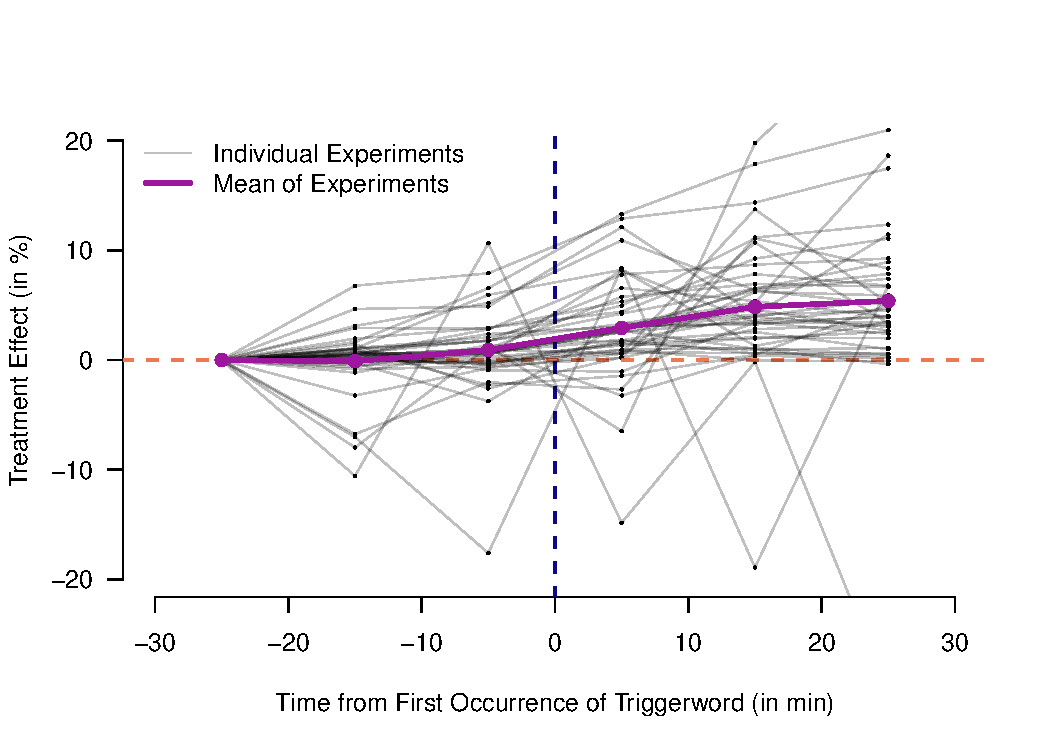
\includegraphics[width=\textwidth]{../figures/triggers/robustness_event_study_H2.pdf}
        \caption{Experiments from H2.}
        \label{fig:image5b}
    \end{subfigure}
    
    \caption{Testing the Parallel Trends Assumption with event studies. Individual studies in grey, their time-wise mean in purple.}
    \label{fig:parallel_trends}
\end{figure*}


\subsection{Computational Resources}
\label{sec:appendix-resources}
An \textit{NVIDIA GeForce RTX 4090} GPU was utilised for the experiments conducted. 170 hours spent for the inference process of sentiment analysis, emotion detection, and hate speech detection models.

\subsection{Selected Reddit Comments}\label{sec:appendix-example}
Below we present a Reddit discussion and how it evolves when the trigger "feminism" appears. The comment containing the trigger is \textbf{bolded}.

\vspace{0.5cm}

\noindent\textbf{WARNING: the following comments contain sensitive and potentially offensive language. Reader discretion is advised.}

\begin{quote}
"This image though..."
\end{quote}

\begin{quote}
"Haunting for us, isn't it? But not for the females."
\end{quote}

\begin{quote}
"Well I'm sure most females would find this horrifying too."
\end{quote}

\begin{quote}
"You a female? Why are you on this Sub?"
\end{quote}

\begin{quote}
\textbf{"Because I'm against feminism?"}
\end{quote}

\begin{quote}
"Well, it's better if these Posts are seen by all the Men out there. Get the taste of true Chameleon female nature."
\end{quote}

\begin{quote}
"Too late. I already saw it."
\end{quote}

\begin{quote}
"There are many women like us on this sub ."
\end{quote}

\begin{quote}
"Yeah I’m a woman and I don’t like it. Women are not a hive mind."
\end{quote}

\begin{quote}
"Women are not a hive mind. You should go out and talk to one maybe."
\end{quote}

\begin{quote}
"My fucking eyes. Sometimes I wish I was blind."
\end{quote}

\begin{quote}
"When Male dies, it's ""sometimes"" sad; when Female dies.............CRIMEEEEE!!!!
\end{quote}

\begin{quote}
"The fucked up world we live in"
\end{quote}
